% Options for packages loaded elsewhere
\PassOptionsToPackage{unicode}{hyperref}
\PassOptionsToPackage{hyphens}{url}
\PassOptionsToPackage{dvipsnames,svgnames,x11names}{xcolor}
%
\documentclass[
  letterpaper,
  DIV=11,
  numbers=noendperiod]{scrartcl}

\usepackage{amsmath,amssymb}
\usepackage{iftex}
\ifPDFTeX
  \usepackage[T1]{fontenc}
  \usepackage[utf8]{inputenc}
  \usepackage{textcomp} % provide euro and other symbols
\else % if luatex or xetex
  \usepackage{unicode-math}
  \defaultfontfeatures{Scale=MatchLowercase}
  \defaultfontfeatures[\rmfamily]{Ligatures=TeX,Scale=1}
\fi
\usepackage{lmodern}
\ifPDFTeX\else  
    % xetex/luatex font selection
\fi
% Use upquote if available, for straight quotes in verbatim environments
\IfFileExists{upquote.sty}{\usepackage{upquote}}{}
\IfFileExists{microtype.sty}{% use microtype if available
  \usepackage[]{microtype}
  \UseMicrotypeSet[protrusion]{basicmath} % disable protrusion for tt fonts
}{}
\makeatletter
\@ifundefined{KOMAClassName}{% if non-KOMA class
  \IfFileExists{parskip.sty}{%
    \usepackage{parskip}
  }{% else
    \setlength{\parindent}{0pt}
    \setlength{\parskip}{6pt plus 2pt minus 1pt}}
}{% if KOMA class
  \KOMAoptions{parskip=half}}
\makeatother
\usepackage{xcolor}
\setlength{\emergencystretch}{3em} % prevent overfull lines
\setcounter{secnumdepth}{-\maxdimen} % remove section numbering
% Make \paragraph and \subparagraph free-standing
\ifx\paragraph\undefined\else
  \let\oldparagraph\paragraph
  \renewcommand{\paragraph}[1]{\oldparagraph{#1}\mbox{}}
\fi
\ifx\subparagraph\undefined\else
  \let\oldsubparagraph\subparagraph
  \renewcommand{\subparagraph}[1]{\oldsubparagraph{#1}\mbox{}}
\fi


\providecommand{\tightlist}{%
  \setlength{\itemsep}{0pt}\setlength{\parskip}{0pt}}\usepackage{longtable,booktabs,array}
\usepackage{calc} % for calculating minipage widths
% Correct order of tables after \paragraph or \subparagraph
\usepackage{etoolbox}
\makeatletter
\patchcmd\longtable{\par}{\if@noskipsec\mbox{}\fi\par}{}{}
\makeatother
% Allow footnotes in longtable head/foot
\IfFileExists{footnotehyper.sty}{\usepackage{footnotehyper}}{\usepackage{footnote}}
\makesavenoteenv{longtable}
\usepackage{graphicx}
\makeatletter
\def\maxwidth{\ifdim\Gin@nat@width>\linewidth\linewidth\else\Gin@nat@width\fi}
\def\maxheight{\ifdim\Gin@nat@height>\textheight\textheight\else\Gin@nat@height\fi}
\makeatother
% Scale images if necessary, so that they will not overflow the page
% margins by default, and it is still possible to overwrite the defaults
% using explicit options in \includegraphics[width, height, ...]{}
\setkeys{Gin}{width=\maxwidth,height=\maxheight,keepaspectratio}
% Set default figure placement to htbp
\makeatletter
\def\fps@figure{htbp}
\makeatother

\usepackage{booktabs}
\usepackage{longtable}
\usepackage{array}
\usepackage{multirow}
\usepackage{wrapfig}
\usepackage{float}
\usepackage{colortbl}
\usepackage{pdflscape}
\usepackage{tabu}
\usepackage{threeparttable}
\usepackage{threeparttablex}
\usepackage[normalem]{ulem}
\usepackage{makecell}
\usepackage{xcolor}
\usepackage[auth-lg]{authblk}
\KOMAoption{captions}{tableheading}
\makeatletter
\@ifpackageloaded{caption}{}{\usepackage{caption}}
\AtBeginDocument{%
\ifdefined\contentsname
  \renewcommand*\contentsname{Table of contents}
\else
  \newcommand\contentsname{Table of contents}
\fi
\ifdefined\listfigurename
  \renewcommand*\listfigurename{List of Figures}
\else
  \newcommand\listfigurename{List of Figures}
\fi
\ifdefined\listtablename
  \renewcommand*\listtablename{List of Tables}
\else
  \newcommand\listtablename{List of Tables}
\fi
\ifdefined\figurename
  \renewcommand*\figurename{Figure}
\else
  \newcommand\figurename{Figure}
\fi
\ifdefined\tablename
  \renewcommand*\tablename{Table}
\else
  \newcommand\tablename{Table}
\fi
}
\@ifpackageloaded{float}{}{\usepackage{float}}
\floatstyle{ruled}
\@ifundefined{c@chapter}{\newfloat{codelisting}{h}{lop}}{\newfloat{codelisting}{h}{lop}[chapter]}
\floatname{codelisting}{Listing}
\newcommand*\listoflistings{\listof{codelisting}{List of Listings}}
\makeatother
\makeatletter
\makeatother
\makeatletter
\@ifpackageloaded{caption}{}{\usepackage{caption}}
\@ifpackageloaded{subcaption}{}{\usepackage{subcaption}}
\makeatother
\ifLuaTeX
  \usepackage{selnolig}  % disable illegal ligatures
\fi
\usepackage{bookmark}

\IfFileExists{xurl.sty}{\usepackage{xurl}}{} % add URL line breaks if available
\urlstyle{same} % disable monospaced font for URLs
\hypersetup{
  pdftitle={PROJETO FINAL - APRENDIZAGEM NÃO SUPERVISIONADA},
  pdfauthor={Pedro Henrique Mello Pereira - 230353025; Bernardo Miguel Esperança Sousa - 230353006; Patricia da Silva Alves Schutz - 230353022},
  colorlinks=true,
  linkcolor={blue},
  filecolor={Maroon},
  citecolor={Blue},
  urlcolor={Blue},
  pdfcreator={LaTeX via pandoc}}

\title{PROJETO FINAL - APRENDIZAGEM NÃO SUPERVISIONADA}
\usepackage{etoolbox}
\makeatletter
\providecommand{\subtitle}[1]{% add subtitle to \maketitle
  \apptocmd{\@title}{\par {\large #1 \par}}{}{}
}
\makeatother
\subtitle{Aplicação de técnivas de Análise dos Componentes Principais e
Análise de Clusters ao conjunto de dados WINE}
\author{Pedro Henrique Mello Pereira - 230353025 \and Bernardo Miguel
Esperança Sousa - 230353006 \and Patricia da Silva Alves Schutz -
230353022}
\date{}

\begin{document}
\maketitle

\renewcommand*\contentsname{Sumário}
{
\hypersetup{linkcolor=}
\setcounter{tocdepth}{3}
\tableofcontents
}
\newpage{}

\section{Secção 1 -
Introdução:}\label{secuxe7uxe3o-1---introduuxe7uxe3o}

Este trabalho tem como objectivo aplicar técnicas de aprendizagem não
supervisionada na análise do data set ``Wine'' disponível no UCI Machine
Learning Repository. Utilizaremos métodos de clusterização, como k-means
e clusterização hierárquica, bem como análise de componentes principais
(PCA) para reduzir a dimensionalidade dos dados e facilitar a
interpretação. O data set ``Wine'' contém 178 amostras de vinho de três
cultivares diferentes, descritas por 13 variáveis que incluem medidas
químicas como acidez, álcool, magnésio e fenóis.

Para determinar o número ideal de clusters, serão utilizadas técnicas
como o silhouette score e a curva de elbow, que ajudam a avaliar a
coesão e a separação dos clusters formados. A padronização dos dados
será considerada para garantir que todas as variáveis contribuam de
maneira equitativa na formação dos clusters. A clusterização hierárquica
será visualizada através de dendrogramas, permitindo uma análise mais
intuitiva das relações hierárquicas entre as amostras de vinho.

A análise de componentes principais (PCA) será empregada como uma
técnica de redução de dimensionalidade, visando identificar as
combinações lineares das variáveis originais que mais explicam a
variância dos dados. O critério de Kaiser (Kaiser criterion) e a
proporção de variância explicada serão utilizados para determinar o
número adequado de componentes principais a serem retidos. Esta etapa é
essencial para simplificar a estrutura dos dados, mantendo a maior
quantidade de informação possível.

Finalmente, os resultados obtidos a partir das diferentes abordagens de
aprendizagem não supervisionada serão comparados e discutidos. Através
desta análise, esperamos identificar padrões e relações subjacentes no
conjunto de dados de vinhos, fornecendo insights valiosos sobre as
características que distinguem os diferentes cultivares. Este estudo
demonstrará a aplicação prática de técnicas de clusterização e PCA,
contribuindo para um melhor entendimento das propriedades dos vinhos
analisados e das técnicas de aprendizagem não supervisionada.

\subsection{Definição dos
objectivos:}\label{definiuxe7uxe3o-dos-objectivos}

A aprendizagem não supervisionada é uma categoria de algoritmos que
busca encontrar padrões e estruturas subjacentes em dados sem o uso de
rótulos ou respostas predefinidas. O principal objectivo deste trabalho
é aplicar essas técnicas para identificar agrupamentos naturais e
padrões no data set ``Wine''.

Especificamente, buscaremos agrupar as amostras de vinho de maneira que
vinhos semelhantes sejam colocados no mesmo cluster, enquanto vinhos
diferentes sejam separados em clusters distintos. Para tanto, testaremos
diferentes técnicas e algoritmos de clusterização como o K-Means e a
Clusterização hierárquica.

Ademais, a análise de componentes principais (ACP) será utilizada com
dois objectivos principais. Primeiro, reduzir a dimensionalidade do
conjunto de dados, facilitando a visualização e interpretação dos
clusters formados. Segundo, identificar as variáveis que mais contribuem
para a variação total dos dados, fornecendo insights sobre as
características mais importantes que diferenciam os vinhos. Esta
abordagem permite simplificar a complexidade dos dados originais sem
perder informações cruciais.

\subsection{Apresentação do conjunto de dados e identificação das
variáveis dependente e
independentes:}\label{apresentauxe7uxe3o-do-conjunto-de-dados-e-identificauxe7uxe3o-das-variuxe1veis-dependente-e-independentes}

O data set ``Wine'' utilizado neste estudo contém 178 amostras de vinho
provenientes de três diferentes cultivares na região da Itália. Cada
amostra é descrita por 13 variáveis químicas que incluem níveis de
acidez, álcool, magnésio, fenóis, entre outros.

A seguir apresentamos o dicionário das variáveis presentes no conjunto
de dados, as quais utilizaremos como como base para a aplicação das
técnicas de clusterização e ACP, a saber:

\begin{itemize}
  \item \textbf{Cultivars}: Tipo ou casta do vinho (1: Barolo, 2: Grignolino, 3: Barbera).
  \item \textbf{Alcohol}: Teor alcoólico do vinho (%).
  \item \textbf{Malic Acid}: Quantidade de ácido málico (g/L).
  \item \textbf{Ash}: Conteúdo de cinzas (g/100mL).
  \item \textbf{Alcalinity of Ash}: Alcalinidade das cinzas (mEq/L).
  \item \textbf{Magnesium}: Quantidade de magnésio (mg/L).
  \item \textbf{Total Phenols}: Quantidade total de fenóis (g/L).
  \item \textbf{Flavanoids}: Quantidade de flavonoides (g/L).
  \item \textbf{Nonflavanoid Phenols}: Quantidade de fenóis não flavonoides (g/L).
  \item \textbf{Proanthocyanins}: Quantidade de proantocianinas (g/L).
  \item \textbf{Color Intensity}: Intensidade da cor do vinho (medida espectrofotométrica).
  \item \textbf{Hue}: Matiz do vinho (medida espectrofotométrica).
  \item \textbf{OD280/OD315 of Diluted Wines}: Razão da absorbância a 280 nm e 315 nm (indicador de compostos fenólicos).
  \item \textbf{Proline}: Quantidade de prolina (mg/L), um aminoácido presente no vinho.
\end{itemize}

\subsubsection{Visão das 5 primeiras entradas do Data set
Wine:}\label{visuxe3o-das-5-primeiras-entradas-do-data-set-wine}

\begingroup\fontsize{3.5}{5.5}\selectfont

\begin{longtable*}{r>{\raggedright\arraybackslash}p{0.5cm}lllrlllllllr}
\toprule
Cultivars & Alcohol & Malic\_Acid & Ash & Ash\_Alcanity & Magnesium & Total\_Phenols & Flavanoids & Nonflavanoid\_Phenols & Proanthocyanins & Color\_Intensity & Hue & OD280 & Proline\\
\midrule
\cellcolor{gray!15}{1} & \cellcolor{gray!15}{14.23} & \cellcolor{gray!15}{1.71} & \cellcolor{gray!15}{2.43} & \cellcolor{gray!15}{15.6} & \cellcolor{gray!15}{127} & \cellcolor{gray!15}{2.8} & \cellcolor{gray!15}{3.06} & \cellcolor{gray!15}{0.28} & \cellcolor{gray!15}{2.29} & \cellcolor{gray!15}{5.64} & \cellcolor{gray!15}{1.04} & \cellcolor{gray!15}{3.92} & \cellcolor{gray!15}{1065}\\
1 & 13.2 & 1.78 & 2.14 & 11.2 & 100 & 2.65 & 2.76 & 0.26 & 1.28 & 4.38 & 1.05 & 3.4 & 1050\\
\cellcolor{gray!15}{1} & \cellcolor{gray!15}{13.16} & \cellcolor{gray!15}{2.36} & \cellcolor{gray!15}{2.67} & \cellcolor{gray!15}{18.6} & \cellcolor{gray!15}{101} & \cellcolor{gray!15}{2.8} & \cellcolor{gray!15}{3.24} & \cellcolor{gray!15}{0.3} & \cellcolor{gray!15}{2.81} & \cellcolor{gray!15}{5.68} & \cellcolor{gray!15}{1.03} & \cellcolor{gray!15}{3.17} & \cellcolor{gray!15}{1185}\\
1 & 14.37 & 1.95 & 2.5 & 16.8 & 113 & 3.85 & 3.49 & 0.24 & 2.18 & 7.8 & 0.86 & 3.45 & 1480\\
\cellcolor{gray!15}{1} & \cellcolor{gray!15}{13.24} & \cellcolor{gray!15}{2.59} & \cellcolor{gray!15}{2.87} & \cellcolor{gray!15}{21} & \cellcolor{gray!15}{118} & \cellcolor{gray!15}{2.8} & \cellcolor{gray!15}{2.69} & \cellcolor{gray!15}{0.39} & \cellcolor{gray!15}{1.82} & \cellcolor{gray!15}{4.32} & \cellcolor{gray!15}{1.04} & \cellcolor{gray!15}{2.93} & \cellcolor{gray!15}{735}\\
\addlinespace
1 & 14.2 & 1.76 & 2.45 & 15.2 & 112 & 3.27 & 3.39 & 0.34 & 1.97 & 6.75 & 1.05 & 2.85 & 1450\\
\bottomrule
\end{longtable*}
\endgroup{}

\subsubsection{Metadados do data set objeto do presente
estudo:}\label{metadados-do-data-set-objeto-do-presente-estudo}

Usando a função ``summary'' do pacote dplyr, explicitaremos um panorama
geral sobre o conjunto de dados em questão, bem como algumas
estatísticas descritivas breves:

\begin{table}[h]
\centering
\begin{tabular}{|c|c|c|c|c|}
\hline
Cultivars & Alcohol & Malic\_Acid & Ash & Ash\_Alcanity \\
\hline
1:59 & Min. :11.03 & Min. :0.740 & Min. :1.360 & Min. :10.60 \\
2:71 & 1st Qu.:12.36 & 1st Qu.:1.603 & 1st Qu.:2.210 & 1st Qu.:17.20 \\
3:48 & Median :13.05 & Median :1.865 & Median :2.360 & Median :19.50 \\
 & Mean :13.00 & Mean :2.336 & Mean :2.367 & Mean :19.49 \\
 & 3rd Qu.:13.68 & 3rd Qu.:3.083 & 3rd Qu.:2.558 & 3rd Qu.:21.50 \\
 & Max. :14.83 & Max. :5.800 & Max. :3.230 & Max. :30.00 \\
\hline
Total\_Phenols & Flavanoids & Nonflavanoid\_Phenols & Proanthocyanins & Color\_Intensity \\
\hline
Min. :0.980 & Min. :0.340 & Min. :0.1300 & Min. :0.410 & Min. : 1.280 \\
1st Qu.:1.742 & 1st Qu.:1.205 & 1st Qu.:0.2700 & 1st Qu.:1.250 & 1st Qu.: 3.220 \\
Median :2.355 & Median :2.135 & Median :0.3400 & Median :1.555 & Median : 4.690 \\
Mean :2.295 & Mean :2.029 & Mean :0.3619 & Mean :1.591 & Mean : 5.058 \\
3rd Qu.:2.800 & 3rd Qu.:2.875 & 3rd Qu.:0.4375 & 3rd Qu.:1.950 & 3rd Qu.: 6.200 \\
Max. :3.880 & Max. :5.080 & Max. :0.6600 & Max. :3.580 & Max. :13.000 \\
\hline
Hue & OD280 & Proline & Magnesium &  \\
\hline
Min. :0.4800 & Min. :1.270 & Min. : 278.0 &  Min. : 70.00 &  \\
1st Qu.:0.7825 & 1st Qu.:1.938 & 1st Qu.: 500.5 & 1st Qu.: 88.00 &  \\
Median :0.9650 & Median :2.780 & Median : 673.5 & Median : 98.00 &  \\
Mean :0.9574 & Mean :2.612 & Mean : 746.9 & Mean : 99.74 &  \\
3rd Qu.:1.1200 & 3rd Qu.:3.170 & 3rd Qu.: 985.0 & 3rd Qu.:107.00 &  \\
Max. :1.7100 & Max. :4.000 & Max. :1680.0 & Max. :162.00 &  \\
\hline
\end{tabular}
\caption{Descrição dos dados.}
\label{tab:dados}
\end{table}

\textbf{Como podemos perceber, trata-se de um data set com poucas
observações, a saber 178 linhas e 14 colunas.}

Quanto à presença de valores nulos, conforme depreende-se da análise da
figura a seguir, o conjunto de dados encontra-se completo e não
apresenta valores nulos ou a preencher, sendo este um importante
indicador a respeito da qualidade dos dados.

\begingroup\fontsize{8}{10}\selectfont

\begin{longtable}[t]{l>{\raggedleft\arraybackslash}p{1cm}}
\caption{\label{tab:unnamed-chunk-3}Contagem de Valores Ausentes}\\
\toprule
Coluna & Valores Ausentes\\
\midrule
\cellcolor{gray!15}{Cultivars} & \cellcolor{gray!15}{0}\\
Alcohol & 0\\
\cellcolor{gray!15}{Malic\_Acid} & \cellcolor{gray!15}{0}\\
Ash & 0\\
\cellcolor{gray!15}{Ash\_Alcanity} & \cellcolor{gray!15}{0}\\
\addlinespace
Magnesium & 0\\
\cellcolor{gray!15}{Total\_Phenols} & \cellcolor{gray!15}{0}\\
Flavanoids & 0\\
\cellcolor{gray!15}{Nonflavanoid\_Phenols} & \cellcolor{gray!15}{0}\\
Proanthocyanins & 0\\
\addlinespace
\cellcolor{gray!15}{Color\_Intensity} & \cellcolor{gray!15}{0}\\
Hue & 0\\
\cellcolor{gray!15}{OD280} & \cellcolor{gray!15}{0}\\
Proline & 0\\
\bottomrule
\end{longtable}
\endgroup{}

Na próxima Secção realizaremos o tratamento dos dados, com vistas a
tornar possível a análise exploratória do conjunto de observações e
posterior aplicação das técnicas de aprendizagem não supervisionada.

\subsection{Secção 2 - Limpeza e Tratamento dos
dados:}\label{secuxe7uxe3o-2---limpeza-e-tratamento-dos-dados}

Em termos de limpeza propriamente dita, não há muito a ser feito haja
vista que os dados são compostos por poucas entradas, não havendo
nulidades ou anomalias aparentes.

Entretanto, é necessário que se realize uma etapa de tratamento dos
dados, o que faremos a partir de então. Como primeira medida, realizamos
a conversão das variáveis para os tipos corretos. A Única coluna do
conjunto de dados que possui o tipo categórico é ``Cultivars''. As
demais são todas numéricas. Desta feita, foi feita a conversão para os
tipos corretos de maneira a evitar problemas mais à frente quando da
standardização dos dados.

Em seguida, atuamos na identificação de possíveis entradas duplicadas no
data set, recebendo como resultado 0 entradas duplicadas, tendo-se
afastado portanto a necessidade de eliminar alguma observção em
duplicidade.

\subsubsection{Busca por outliers:}\label{busca-por-outliers}

Após a etapa de eliminacão de busca porvalores duplicados e correção dos
tipos das variáveis, é importante atentarmo-nos para a existência de
outliers, que são valores que se afastam significativamente da maioria
dos outros valores num conjunto de dados. Eles podem distorcer análises
estatísticas e modelos, de modo a exercer influências indesejadas nos
resultados.

\begin{figure}[H]

{\centering 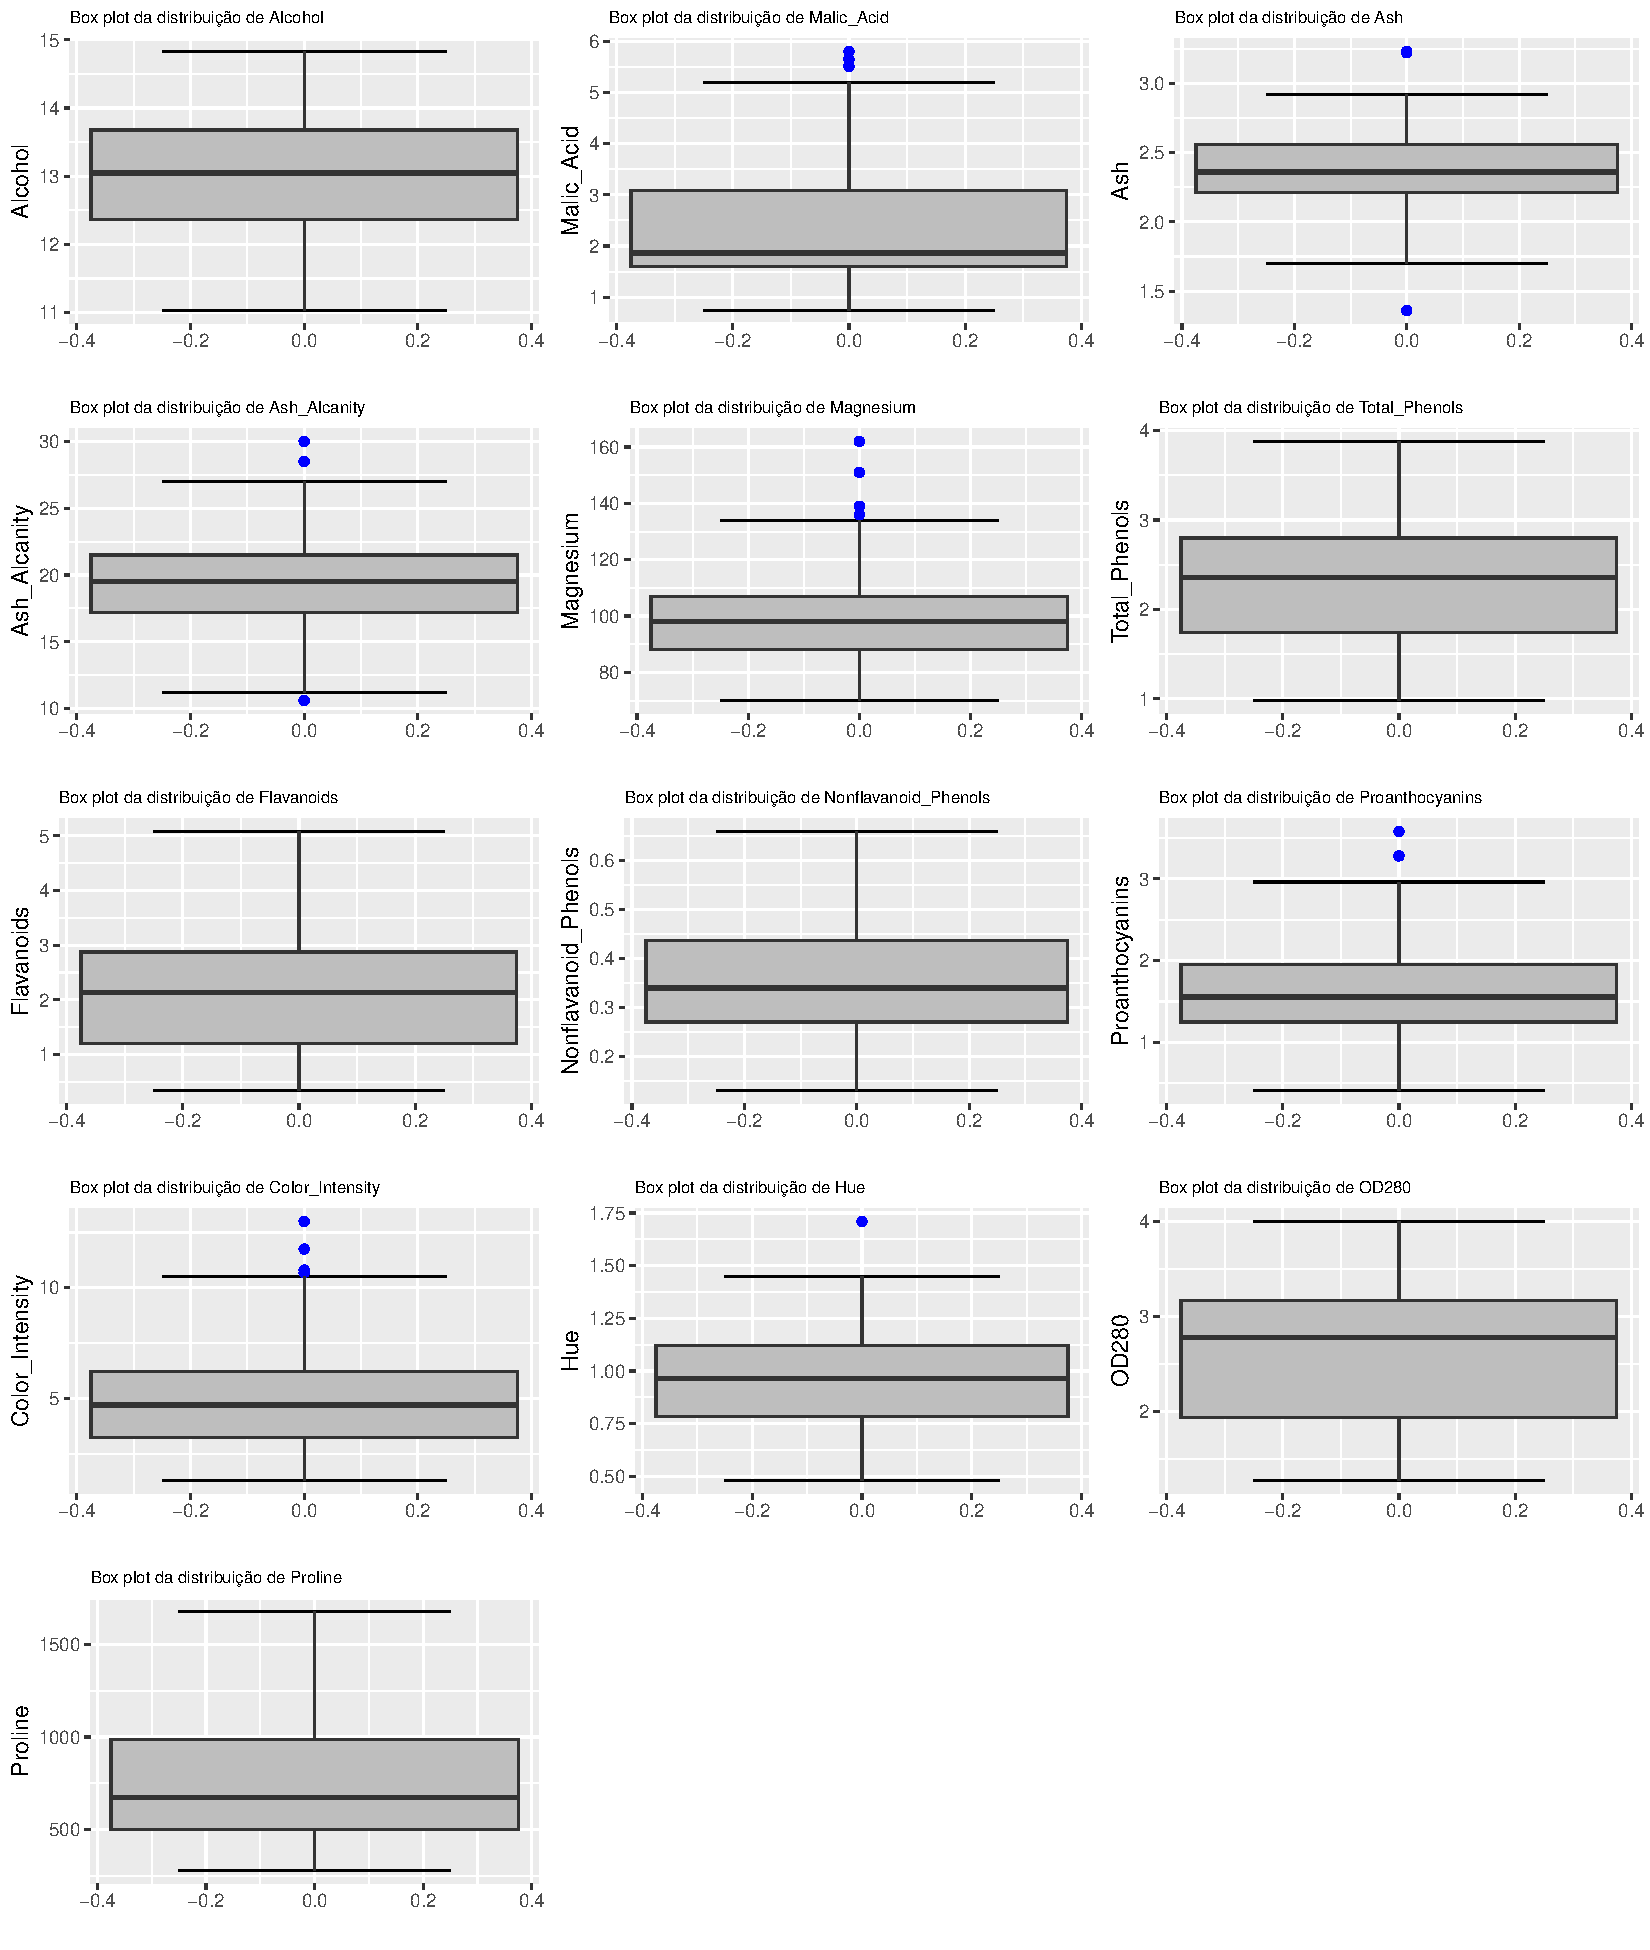
\includegraphics{wines_analysis_files/figure-pdf/unnamed-chunk-5-1.pdf}

}

\caption{Distribuições com Outliers}

\end{figure}%

\newpage{}

Conforme depreende-se da análise dos boxplots, as variáveis `malic
acid', `ash', `ash alcalinity', `magnesium', `Proanthocyanins', `color
intensity' e `hue' apresentaram outliers em sua composição. A presença
de outliers pode representar um risco para a correta execução da análise
de clusters e do ACP, sendo uma boa prática a retirada destes valores.

Entretanto, haja vista ser um data set que possui poucas observações,
optaremos aqui pela não exclusào destes outliers, de modo a não reduzir
ainda mais o universo de observações.

Ademais, em virtude do presente trabalho ser um laboratório para
experimentação, utilizaremos outras técnicas como por exemplo a
regularização dos dados e a comparação entre single/complete/average
linkage para analisar o quão eficazes são no auxílio à regularização
destes valores desviantes.

Após a finalização da limpeza dos dados, vamos salvá-los em um novo
ficheiro o qual chamaremos de ``wine\_clean'' e que será utilizado de
agora em diante na análise exploratória e modelagem.

\subsection{Secção 3 - Análise Exploratória dos
Dados}\label{secuxe7uxe3o-3---anuxe1lise-exploratuxf3ria-dos-dados}

Ao implementar as etapas de limpeza anteriores, criamos um conjunto de
dados mais refinado e confiável, estabelecendo a base para nossa
subsequente análise exploratória de dados (AED), de modo a preparar os
dados para aplicação dos algoritmos de aprendizagem não supervisionada.
O tratamento cuidadoso dos problemas de qualidade dos dados é crucial
para garantir a precisão e confiabilidade dos insights que serão
derivados do conjunto de dados.

Prosseguindo, o foco neste momento será na Análise Exploratória de Dados
(AED) para obter insights mais profundos sobre os diferentes tipos de
vinhos. Esta fase analítica tem como objectivo descobrir tendências
significativas, correlações e padrões dentro do conjunto de dados.

\subsubsection{Matriz de correlação de
Pearson}\label{matriz-de-correlauxe7uxe3o-de-pearson}

Neste momento plotaremos a matriz de correlação de Pearson entre as
variáveis numéricas do data set wine.

A correlação de Pearson é uma medida estatística que avalia a relação
linear entre duas variáveis contínuas. \textbf{Essa medida varia de -1 a
1, onde um valor próximo de 1 indica uma forte correlação positiva, um
valor próximo de -1 indica uma forte correlação negativa e um valor
próximo de 0 indica ausência de correlação linear.} Em outras palavras,
a correlação de Pearson quantifica a direção e a força da relação linear
entre duas variáveis, sendo amplamente utilizada para determinar o grau
de associação entre diferentes conjuntos de dados.

\newpage{}

A ideia aqui é tentar visualizar se existe alguma correlação linear,
seja ela positiva ou negativa, entre as variáveis do conjunto de dados.

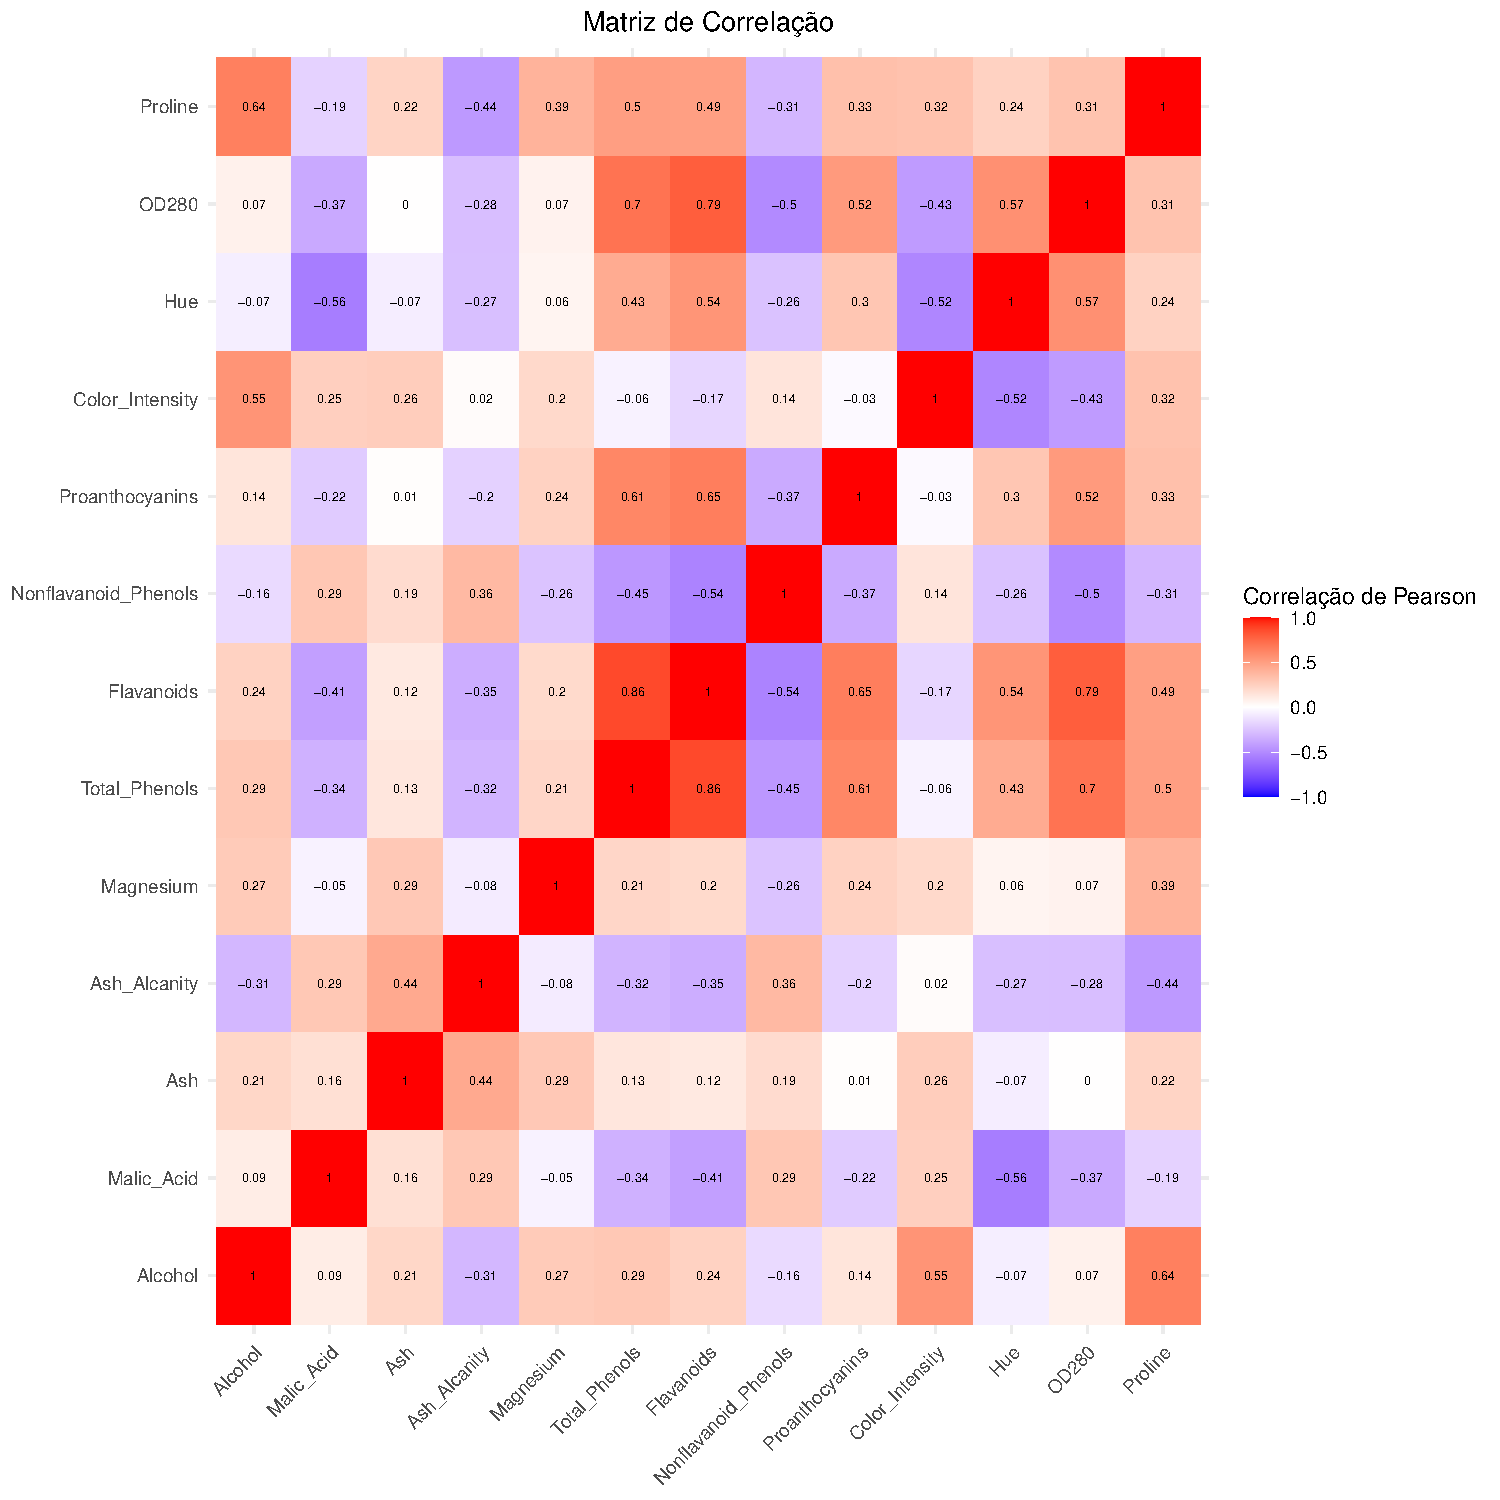
\includegraphics{wines_analysis_files/figure-pdf/unnamed-chunk-7-1.pdf}

\newpage{}

Consideraremos os níveis de correlação encontrados de acordo com a
tabela seguir para balizar a nossa interpretação dos valores:

\begin{longtable}[]{@{}ll@{}}
\toprule\noalign{}
Intervalo de Correlação & Interpretação \\
\midrule\noalign{}
\endhead
\bottomrule\noalign{}
\endlastfoot
-1.0 a -0.71 & Correlação negativa muito forte \\
-0.7 a -0.51 & Correlação negativa forte \\
-0.5 a -0.31 & Correlação negativa moderada \\
-0.3 a -0.11 & Correlação negativa fraca \\
-0.1 a 0 & Correlação negativa muito fraca \\
0 a 0.1 & Correlação positiva muito fraca \\
0.11 a 0.3 & Correlação positiva fraca \\
0.31 a 0.5 & Correlação positiva moderada \\
0.51 a 0.7 & Correlação positiva forte \\
0.71 a 1.0 & Correlação positiva muito forte \\
\end{longtable}

Haja vista tratar-se de um número significativo de variáveis,
comentaremos apenas a respeito daquelas correlações que parecem ser
fortes ou muito fortes, tanto negativas quanto positivas.

Além disso, \textbf{a variável CULTIVARS não será considerada na análise
de correlação por se tratar da única variável categórica existente no
conjunto de dados, não sendo portanto correto analisá-la sob o prisma do
coeficiente de correlação de Pearson.}

\begin{itemize}
\tightlist
\item
  Alcohol: Apresenta correlação linear positiva forte com
  Color\_intensity(0.55) e Proline(0.64), de modo a demonstrar que à
  medida que os valores para uma dessas variáveis aumenta, a outra
  variável também terá um acréscimo em seu valor; De acordo com as
  referências interpretativas definidas neste estudo, a variável em
  questão não apresentou correlação linear negativa forte com nenhum dos
  demais atributos;
\end{itemize}

\begin{center}
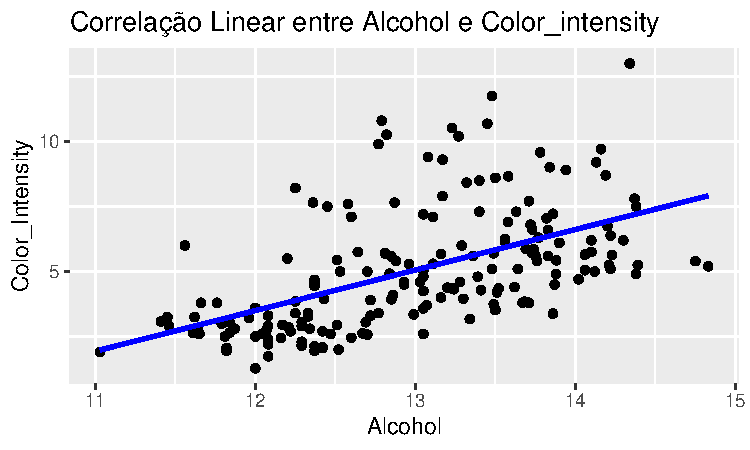
\includegraphics{wines_analysis_files/figure-pdf/unnamed-chunk-8-1.pdf}
\end{center}

\begin{center}
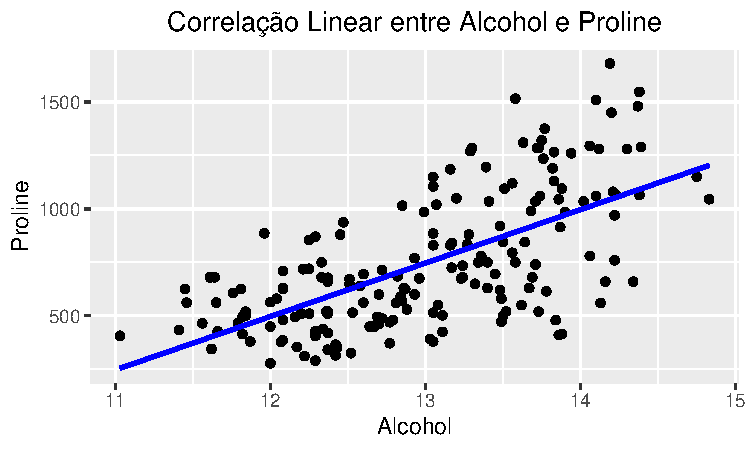
\includegraphics{wines_analysis_files/figure-pdf/unnamed-chunk-8-2.pdf}
\end{center}

\begin{itemize}
\tightlist
\item
  Malic\_Acid: De acordo com as referências interpretativas definidas
  neste estudo, a variável em questão não apresentou correlação linear
  positiva forte com nenhum dos demais atributos; Apresenta correlação
  linear negativa forte com Hue, de -0.56. Isto demonstra que à medida
  que os valores para uma dessas variáveis aumenta, a outra variável
  tende a apresentar uma diminuição em seu valor;
\end{itemize}

\begin{center}
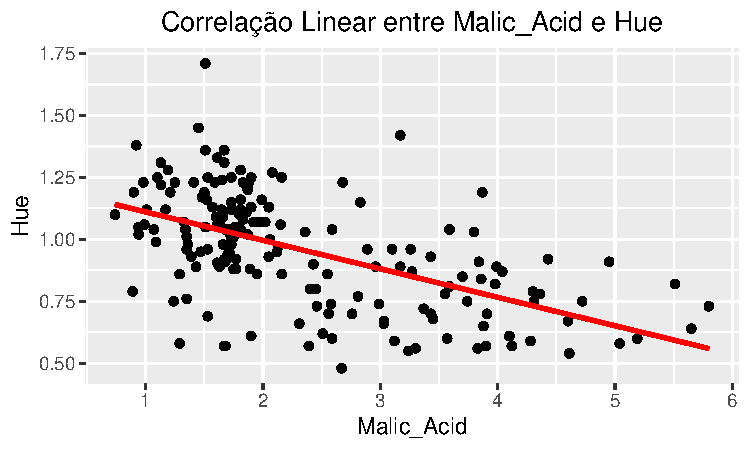
\includegraphics{wines_analysis_files/figure-pdf/unnamed-chunk-9-1.pdf}
\end{center}

\begin{itemize}
\item
  Ash: De acordo com as referências interpretativas definidas neste
  estudo, a variável em questão não apresentou correlação linear
  positiva ou negativa forte com nenhum dos demais atributos;
\item
  Ash\_Alcanity: De acordo com as referências interpretativas definidas
  neste estudo, a variável em questão não apresentou correlação linear
  positiva ou negativa forte com nenhum dos demais atributos;
\item
  Magnesium: De acordo com as referências interpretativas definidas
  neste estudo, a variável em questão não apresentou correlação linear
  positiva ou negativa forte com nenhum dos demais atributos;
\item
  Total\_Phenols: Apresenta correlação linear positiva muito forte com
  Flavanoids, de 0.86, e forte com Proanthocyanins(0.61) e OD280(0.7) de
  modo a demonstrar que à medida que os valores para uma dessas
  variáveis aumenta, a outra variável também terá um acréscimo em seu
  valor; De acordo com as referências interpretativas definidas neste
  estudo, a variável em questão não apresentou correlação linear
  negativa forte com nenhum dos demais atributos;
\end{itemize}

\begin{center}
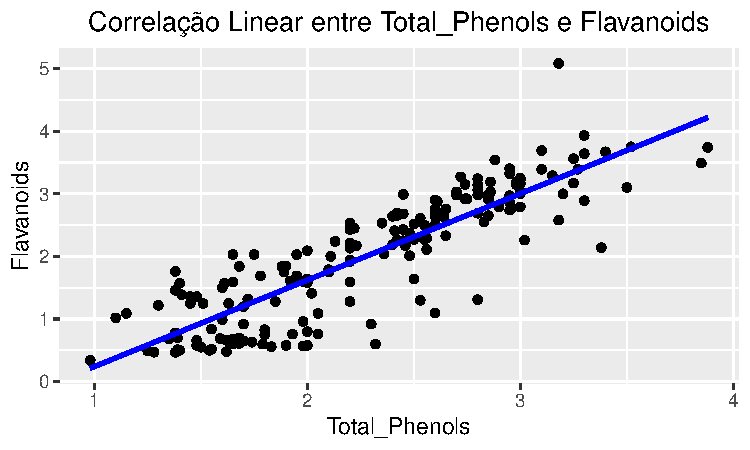
\includegraphics{wines_analysis_files/figure-pdf/unnamed-chunk-10-1.pdf}
\end{center}

\begin{center}
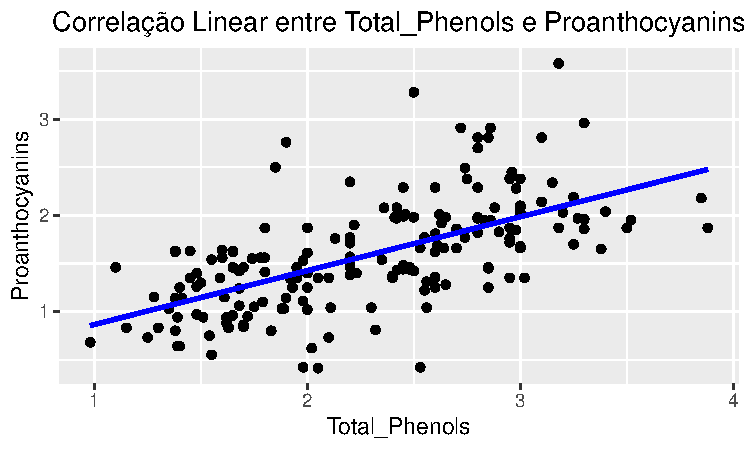
\includegraphics{wines_analysis_files/figure-pdf/unnamed-chunk-10-2.pdf}
\end{center}

\begin{center}
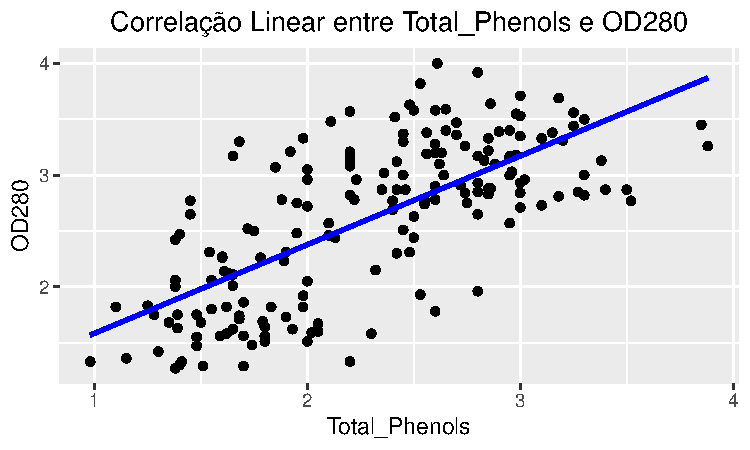
\includegraphics{wines_analysis_files/figure-pdf/unnamed-chunk-10-3.pdf}
\end{center}

\begin{itemize}
\tightlist
\item
  Flavanoids: Conforme demonstrado anteriormente, apresenta correlação
  linear positiva muito forte com Total\_Phenols (0.86) e OD280(0.79),
  Além de forte correlação linear positiva com Proanthocyanins(0.65) e
  Hue(0.54) de modo a demonstrar que à medida que os valores para uma
  dessas variáveis aumenta, a outra variável também terá um acréscimo em
  seu valor; Apresenta correlação linear negativa forte com
  Nonflavanoid\_Phenols, de -0.54. Isto demonstra que à medida que os
  valores para uma dessas variáveis aumenta, a outra variável tende a
  apresentar uma diminuição em seu valor;
\end{itemize}

\begin{center}
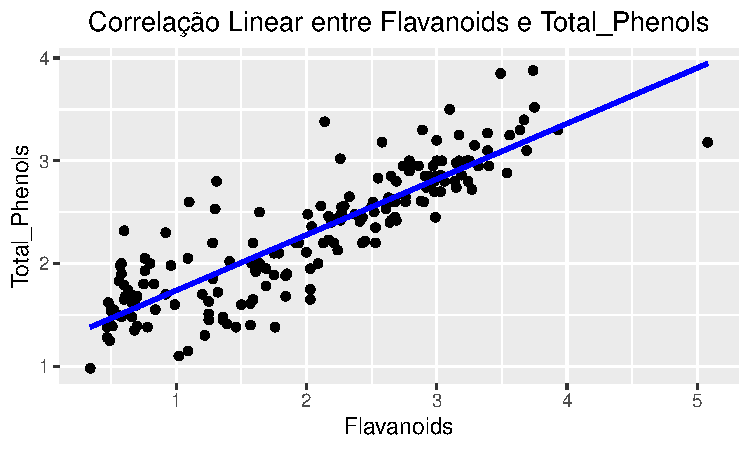
\includegraphics{wines_analysis_files/figure-pdf/unnamed-chunk-11-1.pdf}
\end{center}

\begin{center}
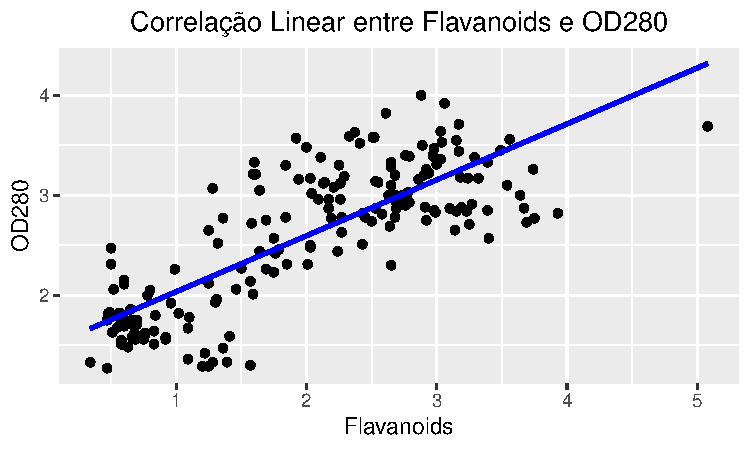
\includegraphics{wines_analysis_files/figure-pdf/unnamed-chunk-11-2.pdf}
\end{center}

\begin{center}
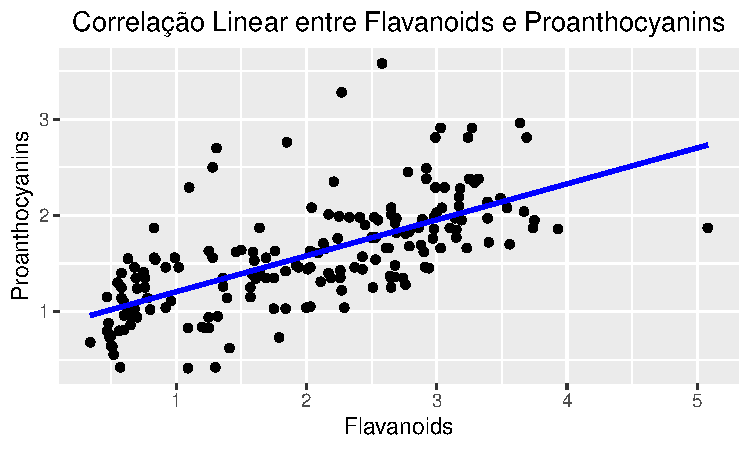
\includegraphics{wines_analysis_files/figure-pdf/unnamed-chunk-11-3.pdf}
\end{center}

\begin{center}
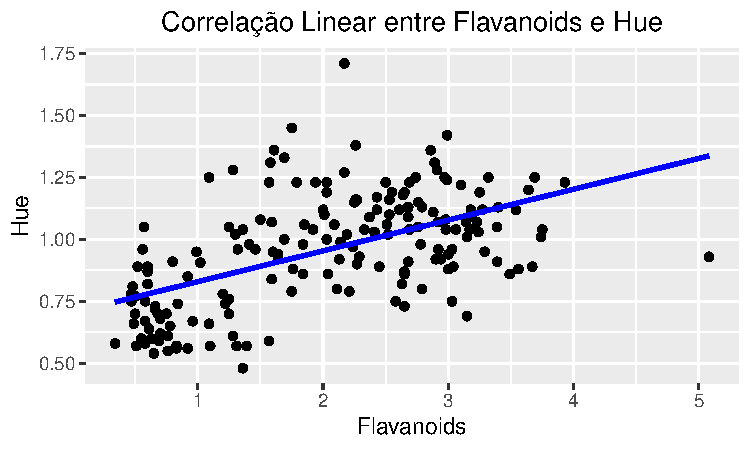
\includegraphics{wines_analysis_files/figure-pdf/unnamed-chunk-11-4.pdf}
\end{center}

\begin{center}
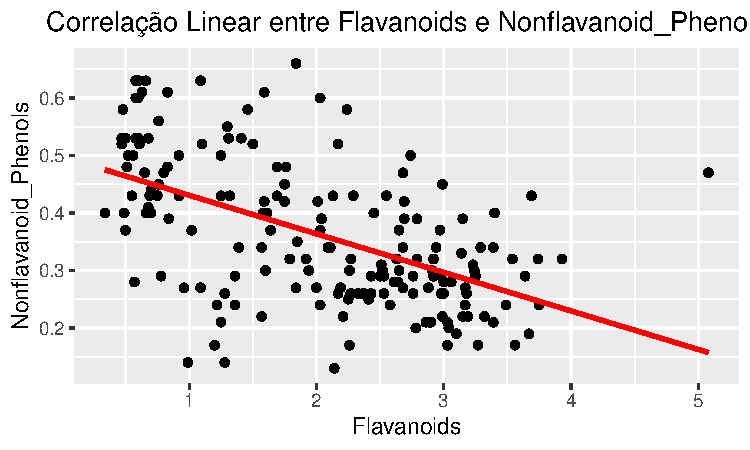
\includegraphics{wines_analysis_files/figure-pdf/unnamed-chunk-11-5.pdf}
\end{center}

\begin{itemize}
\tightlist
\item
  Nonflavanoid\_Phenols: De acordo com as referências interpretativas
  definidas neste estudo, a variável em questão não apresentou
  correlação linear positiva forte com nenhum dos demais atributos;
  Quanto à correlação linear negativa, como era de se esperar em virtude
  de suas naturezas antagônicas, o atributo em questão demonstra uma
  forte correlação linear negativa com a variável flavanoid, de -0.54.
\end{itemize}

\begin{center}
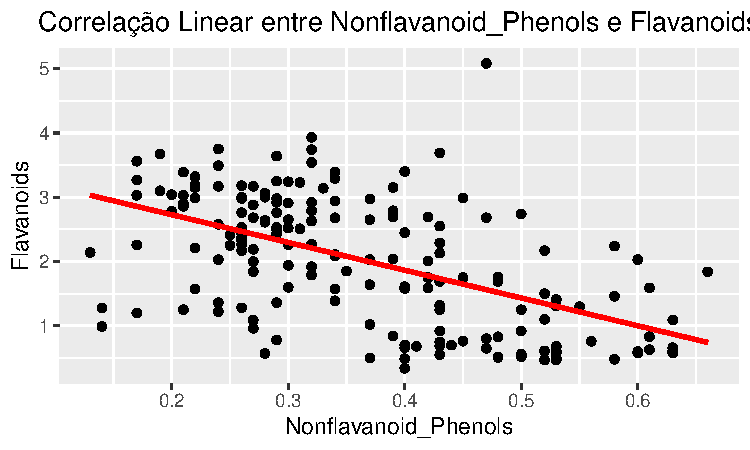
\includegraphics{wines_analysis_files/figure-pdf/unnamed-chunk-12-1.pdf}
\end{center}

\begin{itemize}
\tightlist
\item
  Proanthocyanins: Apresenta correlação linear positiva forte com
  Total\_Phenols (0.61), Flavanoids(0.65) e OD280(0.52), de modo a
  demonstrar que à medida que os valores para uma dessas variáveis
  aumenta, a outra variável também terá um acréscimo em seu valor; De
  acordo com as referências interpretativas definidas neste estudo, a
  variável em questão não apresentou correlação linear negativa forte
  com nenhum dos demais atributos;
\end{itemize}

\begin{center}
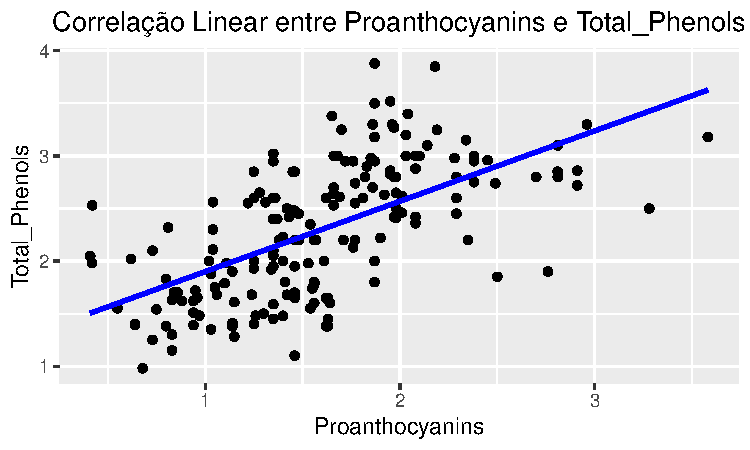
\includegraphics{wines_analysis_files/figure-pdf/unnamed-chunk-13-1.pdf}
\end{center}

\begin{center}
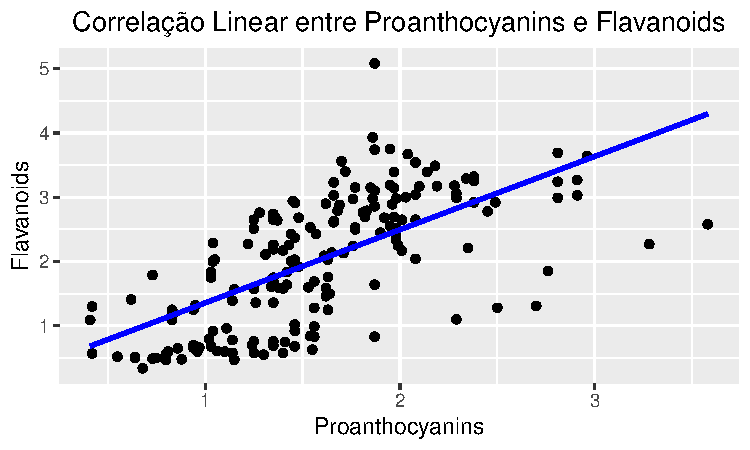
\includegraphics{wines_analysis_files/figure-pdf/unnamed-chunk-13-2.pdf}
\end{center}

\begin{center}
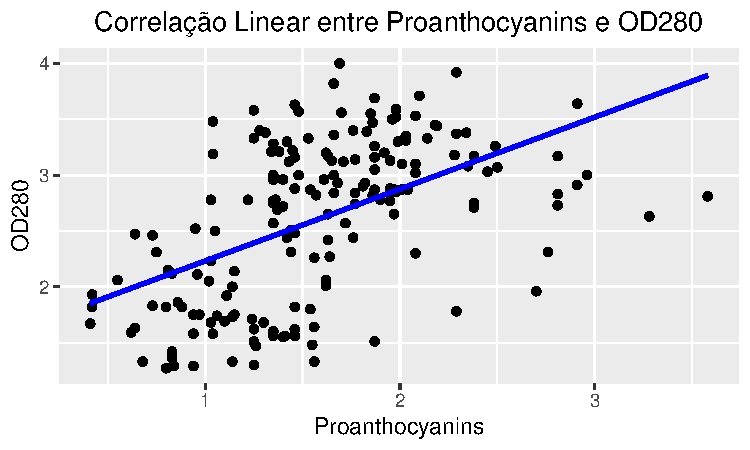
\includegraphics{wines_analysis_files/figure-pdf/unnamed-chunk-13-3.pdf}
\end{center}

\begin{itemize}
\tightlist
\item
  Color\_Intensity: Apresentou forte correlação positiva com Alcohol, de
  0.55, de modo a nos dizer que quanto mais intensa a cor do vinho,
  possivelmente maiorserá o seu teor Alcóolico. De outro modo,
  apresentou correlação linear negativa for (-0.52) com hue, assim sendo
  à medida que os valores para uma dessas variáveis aumenta, a outra
  variável tende a apresentar uma diminuição em seu valor.
\end{itemize}

\begin{center}
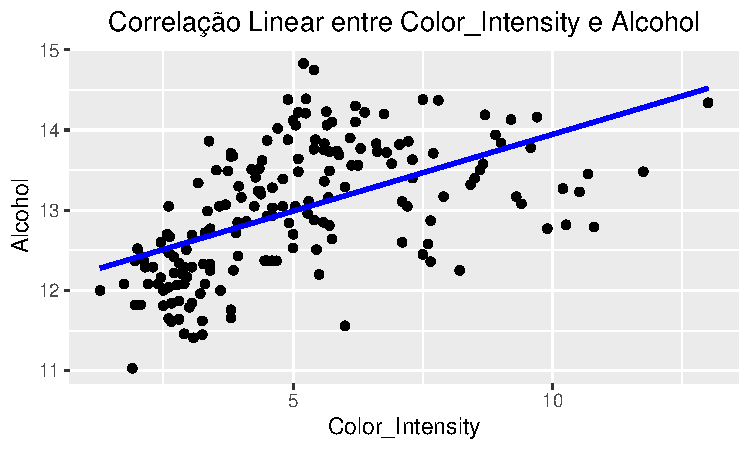
\includegraphics{wines_analysis_files/figure-pdf/unnamed-chunk-14-1.pdf}
\end{center}

\begin{center}
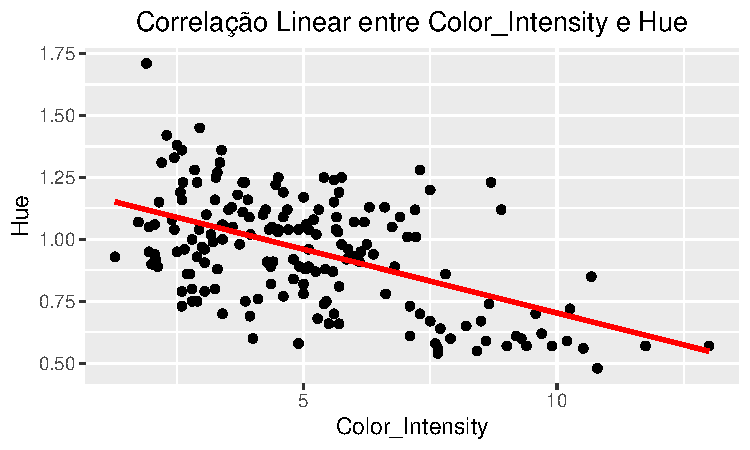
\includegraphics{wines_analysis_files/figure-pdf/unnamed-chunk-14-2.pdf}
\end{center}

\begin{itemize}
\tightlist
\item
  Hue: Apresenta correlação linear positiva forte com Flavanoids(0.54) e
  OD280(0.57), de modo a demonstrar que à medida que os valores para uma
  dessas variáveis aumenta, a outra variável também terá um acréscimo em
  seu valor; Apresenta correlação linear negativa forte com Malic\_Acid,
  de -0.56 e Color\_Intensity, de -0.52. Isto demonstra que à medida que
  os valores para uma dessas variáveis aumenta, a outra variável tende a
  apresentar uma diminuição em seu valor;
\end{itemize}

\begin{center}
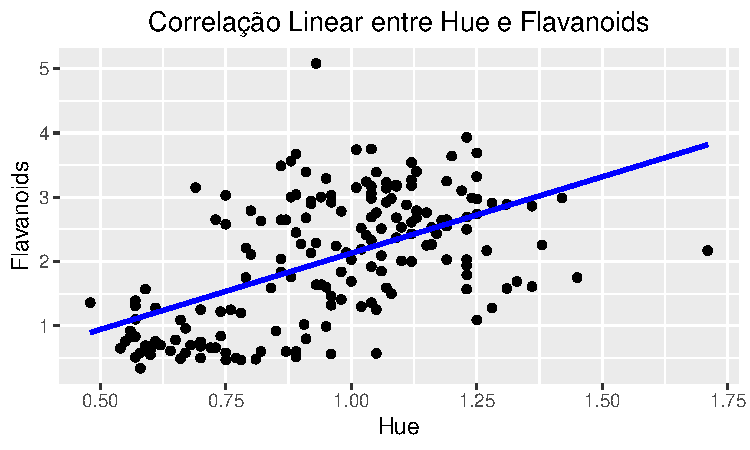
\includegraphics{wines_analysis_files/figure-pdf/unnamed-chunk-15-1.pdf}
\end{center}

\begin{center}
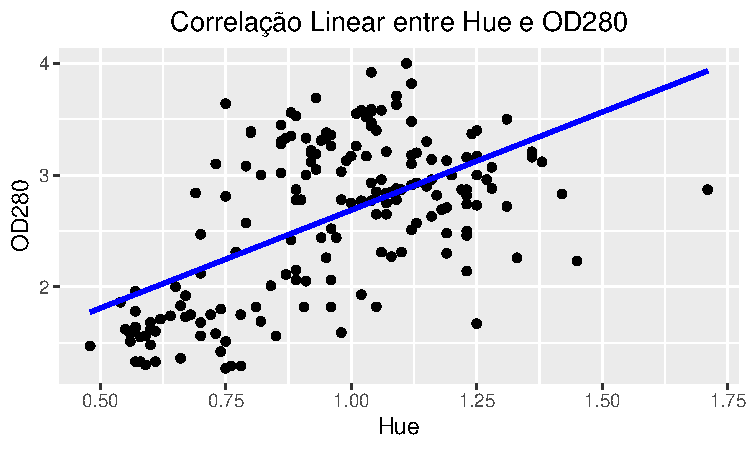
\includegraphics{wines_analysis_files/figure-pdf/unnamed-chunk-15-2.pdf}
\end{center}

\begin{center}
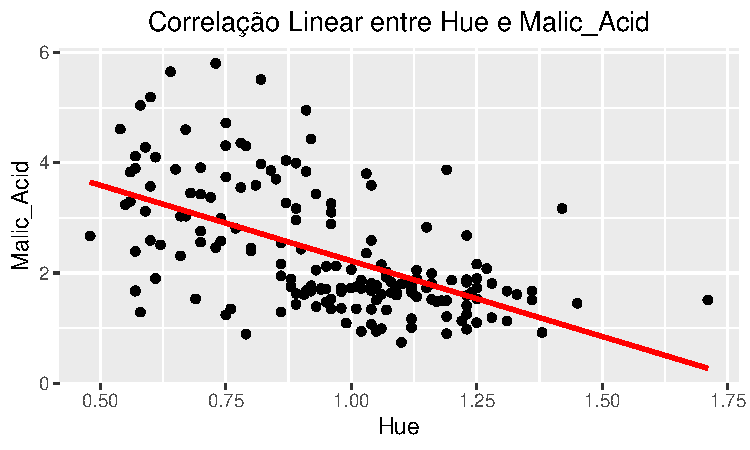
\includegraphics{wines_analysis_files/figure-pdf/unnamed-chunk-15-3.pdf}
\end{center}

\begin{center}
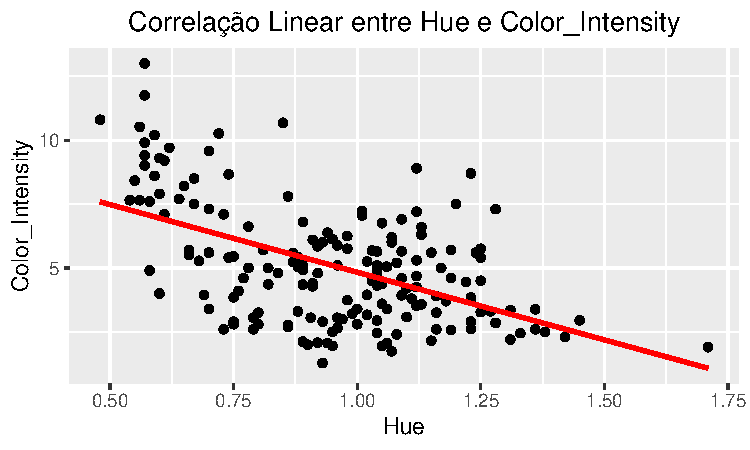
\includegraphics{wines_analysis_files/figure-pdf/unnamed-chunk-15-4.pdf}
\end{center}

\begin{itemize}
\tightlist
\item
  OD280: Apresenta correlação linear positiva forte ou muito forte com
  Total\_Phenols(0.7), Flavanoids(0.79), Proanthocyanins(0.52) e
  Hue(0.57). Isto nos diz que à medida que os valores para uma dessas
  variáveis aumenta, a outra variável também terá um acréscimo em seu
  valor; De acordo com as referências interpretativas definidas neste
  estudo, a variável em questão não apresentou correlação linear
  negativa forte com nenhum dos demais atributos;
\end{itemize}

\begin{center}
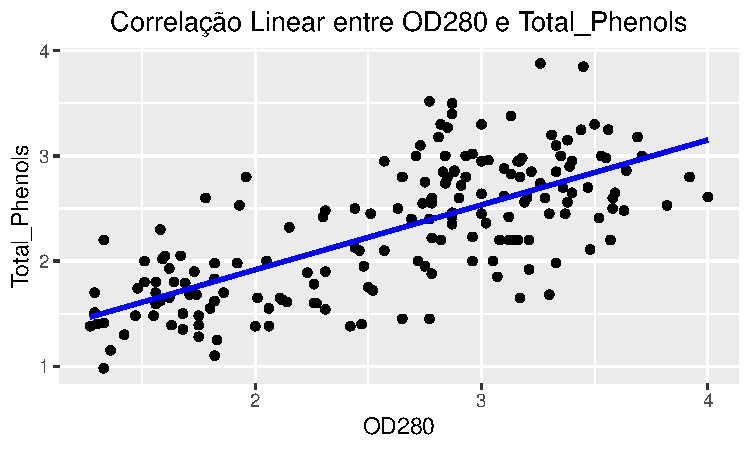
\includegraphics{wines_analysis_files/figure-pdf/unnamed-chunk-16-1.pdf}
\end{center}

\begin{center}
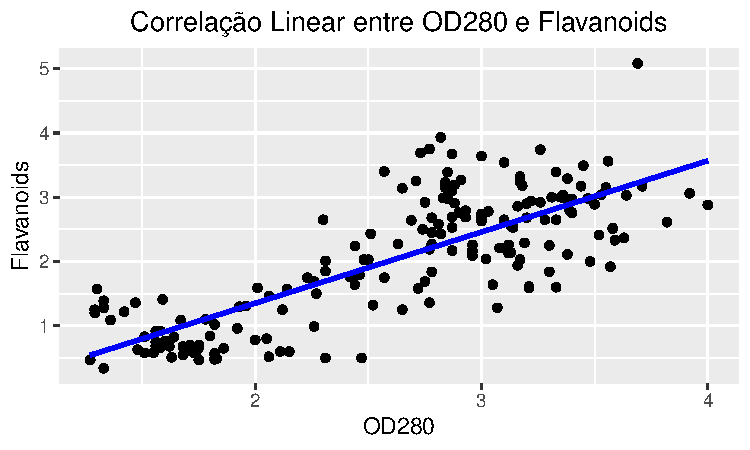
\includegraphics{wines_analysis_files/figure-pdf/unnamed-chunk-16-2.pdf}
\end{center}

\begin{center}
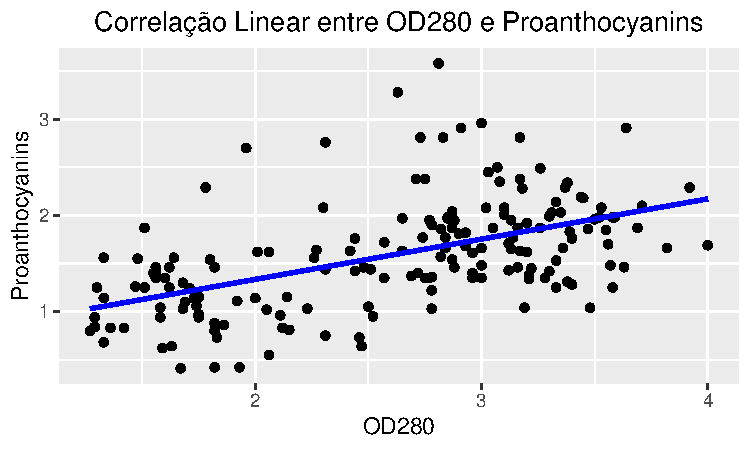
\includegraphics{wines_analysis_files/figure-pdf/unnamed-chunk-16-3.pdf}
\end{center}

\begin{center}
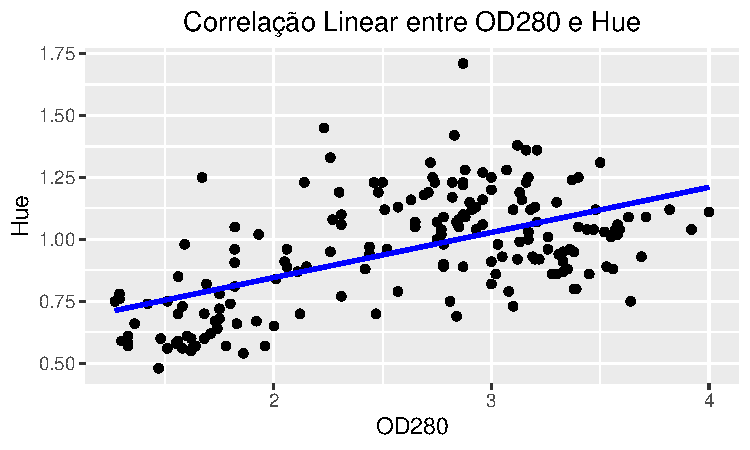
\includegraphics{wines_analysis_files/figure-pdf/unnamed-chunk-16-4.pdf}
\end{center}

\begin{itemize}
\tightlist
\item
  Proline: Demonstrou ter correlação linear positiva forte apenas com o
  atributo Alcohol, no valor de 0.64, de modo a demonstrar que seus
  valores apresentam tendência a serem maiores à medida em que Alcohol
  também é maior. De acordo com as referências interpretativas definidas
  neste estudo, a variável em questão não apresentou correlação linear
  negativa forte com nenhum dos demais atributos;
\end{itemize}

\begin{center}
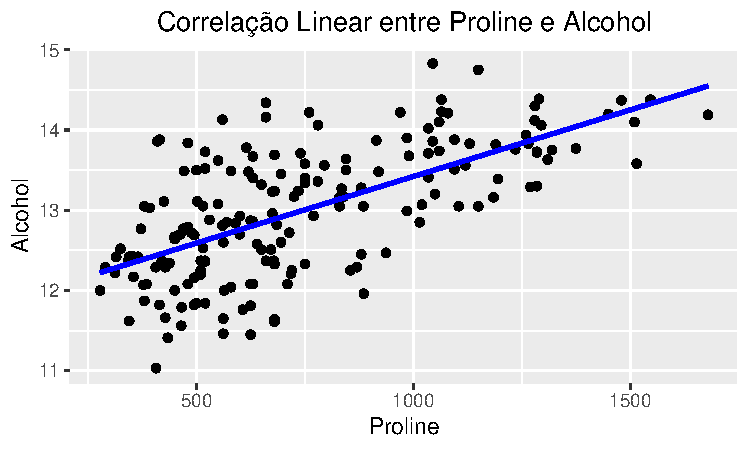
\includegraphics{wines_analysis_files/figure-pdf/unnamed-chunk-17-1.pdf}
\end{center}

\paragraph{Insights importantes advindos das
correlações:}\label{insights-importantes-advindos-das-correlauxe7uxf5es}

Ao analisar as correlações lineares de Pearson entre as variáveis do
conjunto de dados do vinho, é possível extrair insights valiosos sobre
as relações entre suas características químicas que podem auxiliar o
leitor desta análise a escolher um vinho de acordo com estas
características, por exemplo.

A começar pela variável ``Alcohol'', observa-se uma forte correlação
positiva com ``Color\_intensity'' e ``Proline'', sugerindo que vinhos
com teor alcoólico mais elevado tendem a ter uma cor mais intensa e uma
maior concentração de prolina, um aminoácido associado à maturação da
uva. Isso pode indicar uma relação entre a maturação da uva e o teor
alcoólico do vinho, indicando ainda que vinhos com maior concentração
deste aminoácido e teor alcóolico mais elevado podem ser mais doces ao
paladar se comparados aos demais.

Quanto à variável ``Hue'', ela diz respeito à tonalidade do vinho
apresenta correlação linear positiva forte com ``Flavanoids'' e
``OD280'', o que sugere que vinhos com tonalidades mais vibrantes tendem
a ter maiores concentrações de flavonoides e um índice de cor mais
elevado. Por outro lado, ``Hue'' demonstra uma correlação negativa forte
com ``Malic\_Acid'' e ``Color\_Intensity'', indicando que vinhos com
tonalidades mais vibrantes e matizes mais azulados tendem a ter menores
níveis de acidez málica.

Outra observação interessante é a relação entre ``Total\_Phenols'' e
``Flavanoids''. Ambas as variáveis mostram uma correlação positiva muito
forte, o que sugere que vinhos com maiores níveis de fenóis totais
também tendem a ter maiores concentrações de flavonoides. Isso pode
indicar uma relação entre a presença desses compostos e características
sensoriais como aroma, sabor e cor do vinho.

Esses insights fornecem uma compreensão mais profunda das
características químicas dos vinhos apresentados no data set em estudo e
como elas podem relacionar-se entre si, o que pode ser útil para
enólogos e produtores na elaboração e na avaliação da qualidade dos
vinhos, bem como para pessoas que gostariam de escolher vinhos que se
adequem ao seu gosto.

\subsection{Secção 4 - Aplicação de Métodos de Aprendizagem Não
Supervisionada}\label{secuxe7uxe3o-4---aplicauxe7uxe3o-de-muxe9todos-de-aprendizagem-nuxe3o-supervisionada}

Após a conclusão das etapas de preparação dos dados e exploração das
suas principais características, nos concentraremos a partir deste
instante na aplicação de modelos de aprendizagem de máquina não
supervisionados, mais precisamente aqueles denominados como Análise dos
Componentes Principais (ACP) e Análise de Clusters, para aprofundar
ainda mais o conhecimento sobre o conjunto de dados e avançar na busca
de padrões intrínsecos - sobretudo no que diz respeito às melhores
maneiras de se agrupar estes dados e reduzir a dimensionalidade no que
diz respeito ao número de atributos.

A análise dos componentes principais é uma técnica de aprendizagem não
supervisionada utilizada para redução de dimensionalidade e
identificação de padrões nos dados. O PCA busca representar os dados em
um espaço de dimensão menor, preservando a maior parte da variabilidade
original. Isso é feito através da transformação dos dados em um novo
conjunto de variáveis não correlacionadas, chamadas de componentes
principais.

Os componentes principais são ordenados de forma que o primeiro capture
a maior variabilidade nos dados, o segundo capture a segunda maior
variabilidade e assim por diante. O PCA é frequentemente usado para
visualizar a estrutura dos dados em um espaço de dimensão reduzida,
identificar relações entre variáveis e remover redundâncias nos dados.
Ele é especialmente útil quando os dados têm muitas variáveis e queremos
simplificar a análise enquanto mantemos o máximo de informações
possível, sendo este o caso da análise em questão neste trabalho.

A análise de clusters, por sua vez, também pode ser definida como uma
técnica de aprendizagem não supervisionada, sendo útil na tarefa de
encontrar grupos naturais ou ``clusters'' nos dados. O objectivo é
agrupar objetos de tal forma que objetos dentro do mesmo cluster sejam
mais semelhantes entre si do que com objetos de outros clusters. O
algoritmo de clustering atribui os dados a clusters com base em medidas
de semelhança/dissemelhança. O resultado da análise de clusters pode
revelar padrões intrínsecos nos dados, identificar grupos de interesse e
facilitar a compreensão da estrutura subjacente dos dados,
constituindo-se como uma importante ferramenta na análise exploratória
de um conjunto de dados.

Ao longo desta Secção realizaremos uma série de testes com vistas a
aplicar os conhecimentos que foram aprendidos em sala de aula durante o
trimestre na UC de aprendizagem não supervisionada, de modo a maximizar
a eficácia e coerência no uso destes artifícios para melhor representar
e entender o conjunto de dados wine.

Desta feita, o objectivo a partir deste momento é desenvolver uma
análise de clusters que melhor se adeque aos dados - que aqui chamaremos
de wine data set - e para isso passaremos obrigatoriamente por uma etapa
de análise dos componentes principais, para saber se essa abordagem
potencializa os resultados pretendidos na clusterização.

Testaremos ainda a análise de clusters com uso do algoritmo K-Means e a
abordagem hierárquica, com o objectivo de alcançar os melhores
resultados possíveis.

\subsubsection{4.1 - Aplicação da Análise dos Componentes Principais
(ACP):}\label{aplicauxe7uxe3o-da-anuxe1lise-dos-componentes-principais-acp}

A primeira medida a ser empregada diz respeito à aplicação da análise
dos componentes principais aos dados originais, \textbf{à exceção da
variável Cultivars} que será eliminada por conta de sua natureza
qualitativa.

Este passo tem por objectivo utilizar a aplicação da ACP aos dados como
um procedimento anterior à análise de Clusters, de modo a perceber se os
resultados obtidos pela clusterização dos componentes principais são
melhores que aqueles obtidos por meio da aplicação do K-Means ou da
abordagem hierárquica diretamente aos dados.

Neste primeiro momento, faremos uso do artifício de redução de
dimensionalidade aos dados sem centralizá-los ou standarizá-los, e
procederemos à análise dos resultados para saber qual o impacto desta
decisão.

\begin{figure}[H]

{\centering 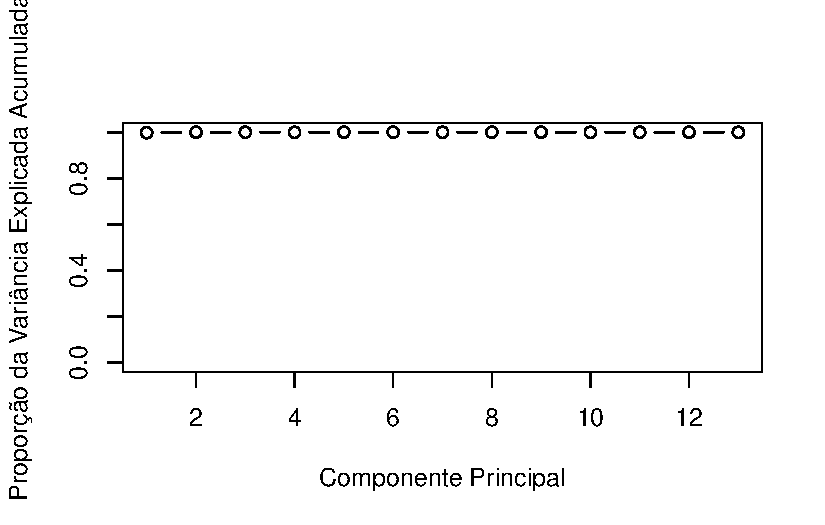
\includegraphics{wines_analysis_files/figure-pdf/unnamed-chunk-18-1.pdf}

}

\caption{Aplicação do ACP aos dados sem centralização e standardização}

\end{figure}%

\textbf{Vejamos o que ocorre na figura:} Como os dados possuem escalas
distintas, a aplicação da centralização e da standardização, que seriam
responsáveis por equalizar o peso dos dados quando do cálculo do ACP, se
mostra fundamental, haja vista que sem isso as variáveis com maior
escala acabam por dominar a análise, de modo a resultar em uma primeira
componente principal que captura a maior parte da variância total.

A tabela a seguir mostra a matriz de rotação das 3 primeiras componentes
principais, onde é possível enxergar a predominância da escala do
componente principal 1 em relação aos demais.

\begin{table}[!h]
\centering
\caption{\label{tab:unnamed-chunk-19}Scores dos Três Primeiros Componentes Principais}
\centering
\resizebox{\ifdim\width>\linewidth\linewidth\else\width\fi}{!}{
\begin{tabular}[t]{>{\raggedleft\arraybackslash}p{3cm}>{\raggedleft\arraybackslash}p{3cm}>{\raggedleft\arraybackslash}p{3cm}}
\toprule
\textbf{PC1} & \textbf{PC2} & \textbf{PC3}\\
\midrule
\cellcolor{gray!10}{-1072.7584} & \cellcolor{gray!10}{-0.9673248} & \cellcolor{gray!10}{8.180732}\\
-1054.6216 & 24.3108121 & 5.766239\\
\cellcolor{gray!10}{-1188.9531} & \cellcolor{gray!10}{37.5913121} & \cellcolor{gray!10}{-1.640828}\\
-1483.2441 & 61.2935580 & 1.007654\\
\cellcolor{gray!10}{-744.1472} & \cellcolor{gray!10}{-32.5753080} & \cellcolor{gray!10}{2.977988}\\
\addlinespace
-1453.2935 & 59.1413091 & 2.602673\\
\bottomrule
\end{tabular}}
\end{table}

\paragraph{4.1.1 - Aplicação da Análise dos Componentes Principais (ACP)
aos dados centralizados e
standardizados:}\label{aplicauxe7uxe3o-da-anuxe1lise-dos-componentes-principais-acp-aos-dados-centralizados-e-standardizados}

\textbf{CENTRALIZAR} os dados significa ajustar cada variável para que
sua média seja igual a zero. Por exemplo, para uma variável \((X)\), a
versão centralizada \((X_{\text{centr}})\) é dada por:

\[ X_{\text{centr}} = X - \bar{X}\]

onde \((\bar{X})\) é a média de \((X)\).

\textbf{STANDARDIZAR} os dados por sua vez vai um passo além da
centralização e ajusta cada variável para que sua média seja zero e seu
desvio padrão seja um. Para uma variável \((X)\), a versão standardizada
\((X_{\text{standard}})\) é dada por:

\[ 
X_{\text{standard}} = \frac{X - \bar{X}}{s_X}
\]

onde \((\bar{X})\) é a média de \((X)\) e \((s_X)\) é o desvio padrão de
\((X)\).

Apresentamos a seguir os resultados da ACP após realização dos
procedimentos retromencionados, a saber:

\begin{figure}[H]

{\centering 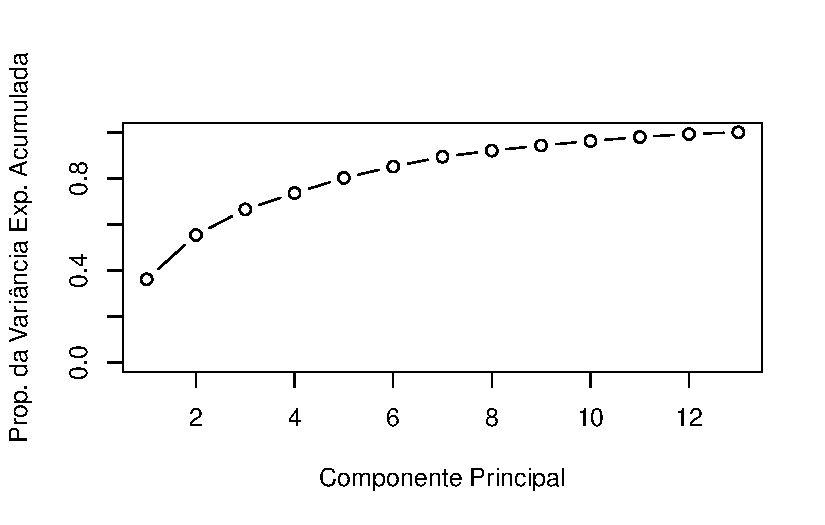
\includegraphics{wines_analysis_files/figure-pdf/unnamed-chunk-20-1.pdf}

}

\caption{Aplicação do ACP aos dados Centralizados e Standardizados}

\end{figure}%

Neste ponto já é possível perceber que houve um salto de qualidade
significativo na aplicação do ACP aos dados padronizados. É possível
observar que a proporção de variância explicada dos dados encontra-se
distribuída ao longo de 13 componentes principais.

Ocorre que a análise dos componentes principais surge como um mecanismo
de redução de dimensionalidade dos dados. Ora, sendo a redução da
dimensionalidade o principal objectivo do uso deste artifício, não faz
sentido reter as 13 componentes principais, haja vista que isto seria
equivalente ao número de colunas do data set (excetuando-se Cultivars
que foi eliminada neste ponto) e portanto não nos auxiliaria.

Soma-se a isso o fato de que alguns componentes principais, nomeadamente
do 8 em diante, não possuem percentual expressivo de proporção de
variância explicada para os dados apresentados, conforme podemos
depreender da análise do screeplot a seguir:

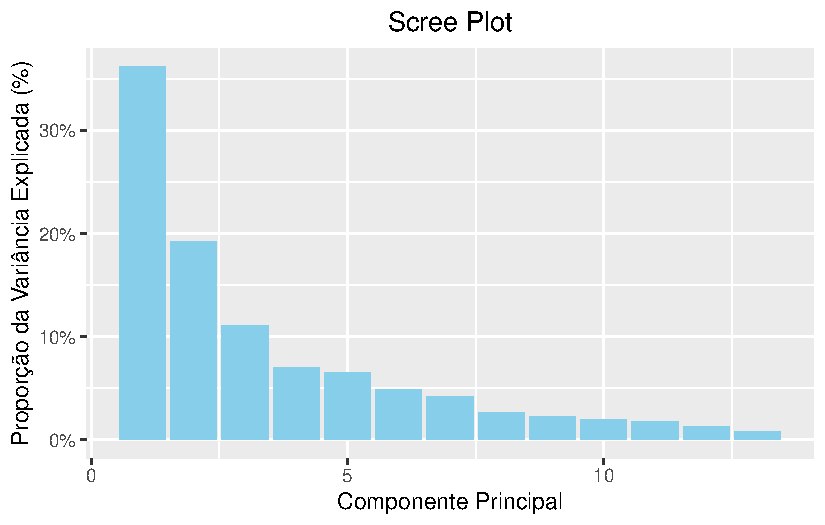
\includegraphics{wines_analysis_files/figure-pdf/unnamed-chunk-21-1.pdf}

\paragraph{Escolha do número de Componentes Principais que serão
retidos:}\label{escolha-do-nuxfamero-de-componentes-principais-que-seruxe3o-retidos}

Demonstramos anteriormente a razão de não haver utilidade em reter todos
os componentes gerados pelo modelo. Desta feita, surge então a
necessidade de decidir quantos componentes principais serão retidos na
análise.

Para tanto, por mais discricionário que pareça, existem métodos que
podem nortear esta escolha de modo a auxiliar o cientista de dados
quando da aplicação da ACP.

\textbf{Método 1: Critério de Kaiser}

Este critério sugere reter apenas os componentes principais que
apresentem variância maior ou igual a 1. Segundo este critério, isto
indica que o componente retém mais variância do que qualquer variável
original padronizada, o que implica que ele contribui significativamente
para explicar a variância total dos dados.

\textbf{Método 2: Análise da Proporção de Variância Explicada Acumulada}
Conforme veremos na tabela a seguir, ao optarmos pelo critério de Kaiser
não seria aconselhável reter mais do que as 3 primeiras componentes
principais no caso em tela. Desta feita, optaremos neste estudo pela
utilização do método de retenção de componentes principais de acordo com
a proporção de variância explicada que cada uma tem.

Isto posto, se optassemos por reter apenas as 3 primeiras componentes
principais - o que seria aconselhável caso fossemos utilizar o critério
de Kaiser - teríamos apenas 66\% da vari6ancia total do conjunto de
dados sendo explicada pelos nossos componentes principais, o que nos
parece pouco e poderia levar-nos a perder uma parte significativa dos
padrões e insights presentes nos dados.

\begin{table}[!h]
\centering
\caption{\label{tab:unnamed-chunk-22}Proporção da Variância Explicada por Componente Principal}
\centering
\resizebox{\ifdim\width>\linewidth\linewidth\else\width\fi}{!}{
\begin{tabular}[t]{>{\raggedright\arraybackslash}p{3cm}>{\raggedleft\arraybackslash}p{3cm}>{\raggedleft\arraybackslash}p{3cm}>{\raggedleft\arraybackslash}p{3cm}}
\toprule
\textbf{ } & \textbf{Variancia} & \textbf{Prop\_Var\_Exp} & \textbf{Prop\_Var\_Exp\_Acum}\\
\midrule
\cellcolor{gray!10}{PC1} & \cellcolor{gray!10}{4.7058503} & \cellcolor{gray!10}{0.36199} & \cellcolor{gray!10}{0.36199}\\
PC2 & 2.4969737 & 0.19207 & 0.55406\\
\cellcolor{gray!10}{PC3} & \cellcolor{gray!10}{1.4460720} & \cellcolor{gray!10}{0.11124} & \cellcolor{gray!10}{0.66530}\\
PC4 & 0.9189739 & 0.07069 & 0.73599\\
\cellcolor{gray!10}{PC5} & \cellcolor{gray!10}{0.8532282} & \cellcolor{gray!10}{0.06563} & \cellcolor{gray!10}{0.80162}\\
\addlinespace
PC6 & 0.6416570 & 0.04936 & 0.85098\\
\cellcolor{gray!10}{PC7} & \cellcolor{gray!10}{0.5510283} & \cellcolor{gray!10}{0.04239} & \cellcolor{gray!10}{0.89337}\\
PC8 & 0.3484974 & 0.02681 & 0.92018\\
\cellcolor{gray!10}{PC9} & \cellcolor{gray!10}{0.2888799} & \cellcolor{gray!10}{0.02222} & \cellcolor{gray!10}{0.94240}\\
PC10 & 0.2509025 & 0.01930 & 0.96170\\
\addlinespace
\cellcolor{gray!10}{PC11} & \cellcolor{gray!10}{0.2257886} & \cellcolor{gray!10}{0.01737} & \cellcolor{gray!10}{0.97907}\\
PC12 & 0.1687702 & 0.01298 & 0.99205\\
\cellcolor{gray!10}{PC13} & \cellcolor{gray!10}{0.1033779} & \cellcolor{gray!10}{0.00795} & \cellcolor{gray!10}{1.00000}\\
\bottomrule
\end{tabular}}
\end{table}

Logo, ao optarmos pelo método de maximização da proporção de variância
explicada, que nos parece mais razoável ao caso em tela,
\textbf{gostaríamos de obter ao menos 80\% da variância total dos dados
dentro das componentes principais definidas}, o que nos leva a um número
mínimo de 5 PC's.

Entretanto, \textbf{o número de 6 PC's também nos parece razoável haja
vista a proporção de variância explicada acumulada ser de 85\% neste
ponto, motivo pelo qual faremos a opção por reter 6 PC's.}

\subparagraph{Matriz de Loadings para a solução
proposta:}\label{matriz-de-loadings-para-a-soluuxe7uxe3o-proposta}

Haja vista termos em consideração como solução escolhida a retenção dos
6 primeiros componentes principais, não sendo tão esclarecedor realizar
a demonstração de um biplot por termos mais do que 2 eixos,
apresentaremos a seguir uma tabela com a matriz de loadings de cada um
em relação às variáveis do data set, para análise e conclusões, de modo
a facilitar a interpretação dos componentes principais em relação aos
dados.

A matriz de rotação(loadings) a seguir mostra como cada variável
contribui para cada componente principal:

\begin{table}[!h]
\centering
\caption{\label{tab:unnamed-chunk-23}Componentes Principais}
\centering
\resizebox{\ifdim\width>\linewidth\linewidth\else\width\fi}{!}{
\begin{tabular}[t]{>{\raggedright\arraybackslash}p{3cm}>{\raggedleft\arraybackslash}p{3cm}>{\raggedleft\arraybackslash}p{3cm}>{\raggedleft\arraybackslash}p{3cm}>{\raggedleft\arraybackslash}p{3cm}>{\raggedleft\arraybackslash}p{3cm}>{\raggedleft\arraybackslash}p{3cm}}
\toprule
\textbf{ } & \textbf{PC1} & \textbf{PC2} & \textbf{PC3} & \textbf{PC4} & \textbf{PC5} & \textbf{PC6}\\
\midrule
\cellcolor{gray!10}{Alcohol} & \cellcolor{gray!10}{-0.1443294} & \cellcolor{gray!10}{-0.4836515} & \cellcolor{gray!10}{-0.2073826} & \cellcolor{gray!10}{-0.0178563} & \cellcolor{gray!10}{0.2656637} & \cellcolor{gray!10}{-0.2135386}\\
Malic\_Acid & 0.2451876 & -0.2249309 & 0.0890129 & 0.5368903 & -0.0352136 & -0.5368138\\
\cellcolor{gray!10}{Ash} & \cellcolor{gray!10}{0.0020511} & \cellcolor{gray!10}{-0.3160688} & \cellcolor{gray!10}{0.6262239} & \cellcolor{gray!10}{-0.2141756} & \cellcolor{gray!10}{0.1430255} & \cellcolor{gray!10}{-0.1544747}\\
Ash\_Alcanity & 0.2393204 & 0.0105905 & 0.6120803 & 0.0608594 & -0.0661029 & 0.1008245\\
\cellcolor{gray!10}{Magnesium} & \cellcolor{gray!10}{-0.1419920} & \cellcolor{gray!10}{-0.2996340} & \cellcolor{gray!10}{0.1307569} & \cellcolor{gray!10}{-0.3517966} & \cellcolor{gray!10}{-0.7270485} & \cellcolor{gray!10}{-0.0381439}\\
\addlinespace
Total\_Phenols & -0.3946608 & -0.0650395 & 0.1461790 & 0.1980683 & 0.1493184 & 0.0841223\\
\cellcolor{gray!10}{Flavanoids} & \cellcolor{gray!10}{-0.4229343} & \cellcolor{gray!10}{0.0033598} & \cellcolor{gray!10}{0.1506819} & \cellcolor{gray!10}{0.1522948} & \cellcolor{gray!10}{0.1090258} & \cellcolor{gray!10}{0.0189200}\\
Nonflavanoid\_Phenols & 0.2985331 & -0.0287795 & 0.1703682 & -0.2033010 & 0.5007030 & 0.2585940\\
\cellcolor{gray!10}{Proanthocyanins} & \cellcolor{gray!10}{-0.3134295} & \cellcolor{gray!10}{-0.0393017} & \cellcolor{gray!10}{0.1494543} & \cellcolor{gray!10}{0.3990565} & \cellcolor{gray!10}{-0.1368598} & \cellcolor{gray!10}{0.5337954}\\
Color\_Intensity & 0.0886167 & -0.5299957 & -0.1373062 & 0.0659257 & 0.0764368 & 0.4186441\\
\addlinespace
\cellcolor{gray!10}{Hue} & \cellcolor{gray!10}{-0.2967146} & \cellcolor{gray!10}{0.2792351} & \cellcolor{gray!10}{0.0852219} & \cellcolor{gray!10}{-0.4277714} & \cellcolor{gray!10}{0.1736145} & \cellcolor{gray!10}{-0.1059827}\\
OD280 & -0.3761674 & 0.1644962 & 0.1660046 & 0.1841207 & 0.1011610 & -0.2658511\\
\cellcolor{gray!10}{Proline} & \cellcolor{gray!10}{-0.2867522} & \cellcolor{gray!10}{-0.3649028} & \cellcolor{gray!10}{-0.1267459} & \cellcolor{gray!10}{-0.2320709} & \cellcolor{gray!10}{0.1578688} & \cellcolor{gray!10}{-0.1197256}\\
\bottomrule
\end{tabular}}
\end{table}

Aqui observa-se o seguinte:

\textbf{PC1}: - \texttt{Flavanoids}, \texttt{Total\_Phenols} e
\texttt{ODB280} estão mais fortemente relacionados a este componente,
pois têm os maiores valores absolutos.

Todos os valores são negativos, sugerindo que à medida que o PC1
aumenta, a concentração de flavonoides e fenóis totais tende a diminuir,
assim como o ODB280.

\textbf{PC2}: - \texttt{Alcohol}, \texttt{Color\_Intensity} e
\texttt{Proline} estão mais fortemente relacionadas a este componente,
com os maiores valores absolutos.

Aqui os valores são negativos, sugerindo que à medida que o PC2 aumenta,
a concentração de álcool tende a diminuir, bem como a intensidade da cor
e a concentração de Prolina, o que corrobora com aquilo que fora
apontado na análise exploratória da Secção 3.

\textbf{PC3}: - \texttt{Ash} e \texttt{Ash\_Alcanity} estão mais
fortemente relacionadas a este componente, com os maiores valores
absolutos. Isso sugere que à medida que o PC3 aumenta, ambas também
devem aumentar.

\textbf{PC4}: - \texttt{Malic\_Acid} está mais fortemente relacionado a
este componente, com o maior valor absoluto.

Este valor é positivo, sugerindo que à medida que o PC4 aumenta, a
concentração de Malic Acid tende a aumentar.

\begin{itemize}
\tightlist
\item
  \texttt{Hue} também está mais fortemente relacionado a este
  componente, e apresenta valor negativo, o que nos diz que à medida em
  que PC4 aumenta, a intensidade da tonalidade do vinho tende a
  diminuir;
\end{itemize}

\textbf{PC5}: - \texttt{Magnesium} está mais fortemente relacionado a
este componente, com o maior valor absoluto.

Este valor é negativo, sugerindo que à medida que o PC5 aumenta, a
concentração de magnésio tende a diminuir.

\begin{itemize}
\tightlist
\item
  \texttt{Nonflavanoid\_Phenols} também encontra-se fortemente
  relacionada ao PC5, o que nos diz que à medida em que PC5 aumenta,
  Nonflavanoid\_Phenols deve diminuir.
\end{itemize}

\textbf{PC6}: - \texttt{Proanthocyanins} está mais fortemente
relacionado a este componente, com o maior valor absoluto.

Este valor é positivo, sugerindo que à medida que o PC6 aumenta, a
concentração de proantocianidinas tende a aumentar.

\subsubsection{4.2 - Aplicação da Análise de
Clusters:}\label{aplicauxe7uxe3o-da-anuxe1lise-de-clusters}

De agora em diante nos concentraremos na aplicação da análise de
clusters com vistas a encontrar o melhor segmentação para os dados, de
modo a agrupar vinhos semelhantes e criar grupos com bons valores de
coesão interna e o mais distantes possíveis dos demais.

\paragraph{4.2.1 - Aplicação da Análise de Clusters aos componentes
principais gerados
anteriomente:}\label{aplicauxe7uxe3o-da-anuxe1lise-de-clusters-aos-componentes-principais-gerados-anteriomente}

O primeiro teste que faremos será a utilização dos componentes
principais oriundos dos dados originais, conforme tratamento efetuado na
Secção anterior deste relatório, com o fito de posteriormente comparar o
agrupamento dos componentes principais com o agrupamento dos dados
originais e perceber qual técnica foi a mais adequada ao caso em tela.

Para esta parte da análise, utilizaremos os componentes principais
advindos de pca1, os quais serão armazenados aqui em uma variável
chamada pca\_data. É salutar ressaltar que teremos em consideração
apenas os 6 Componentes Principais que decidimos reter, os quais serão
utilizados na análise de clusters proposta.

\paragraph{4.2.1.1 - Aplicação do K-Means aos componentes
principais:}\label{aplicauxe7uxe3o-do-k-means-aos-componentes-principais}

Sabemos que existem diversas técnicas de análise de clusters, por isso
nos manteremos fieis àquelas que foram ensinadas e aplicadas em sala de
aula.

A primeira delas - e que utilizaremos agora - é o K-Means. Trata-se de
um algoritmo de clustering amplamente utilizado em análise de dados e
aprendizado de máquina para particionar um conjunto de observações em
\(( k )\) clusters. Cada observação pertence ao cluster cujo centro
(centroide) está mais próximo, servindo como um protótipo do cluster. O
objectivo é minimizar a variabilidade dentro de cada cluster, medida
pela soma das distâncias quadradas entre cada ponto e o centroide do seu
cluster. O valor de \(( k )\), que é o número de clusters desejado, deve
ser especificado pelo usuário sendo esta uma das ``desvantagens'' da
aplicação do K-Means em relação à abordagem hierárquica, que também será
aplicada oportunamente nesta análise. Entretanto, esta desvantagem pode
ser mitigada pelo uso de métodos como a curva do elbow ou o silhouette
score.

\subparagraph{\texorpdfstring{\textbf{Definição do número ideal de
clusters por meio da aplicação das técnicas do silhouette score e curva
de
elbow.}}{Definição do número ideal de clusters por meio da aplicação das técnicas do silhouette score e curva de elbow.}}\label{definiuxe7uxe3o-do-nuxfamero-ideal-de-clusters-por-meio-da-aplicauxe7uxe3o-das-tuxe9cnicas-do-silhouette-score-e-curva-de-elbow.}

A \textbf{curva do cotovelo (elbow curve)} é um método gráfico usado
para determinar o número ideal de clusters numa análise de clustering.
Ao aplicar o k-means, calcula-se a soma das distâncias quadradas dentro
dos clusters (Within-Cluster Sum of Squares, WSS) para diferentes
valores de \(( k )\). Os valores de WSS são plotados contra o número de
clusters. O ponto onde há uma diminuição abrupta na inclinação da curva
é chamado de elbow (cotovelo em tradução livre) e indica o número
apropriado de clusters, onde adicionar mais clusters além deste ponto
não resulta numa redução significativa na variabilidade interna dos
clusters.

O \textbf{silhouette score} é uma métrica que avalia a qualidade dos
clusters formados. Para cada ponto, calcula-se a diferença entre a
distância média para os pontos do mesmo cluster \((a)\) e a distância
média para os pontos do cluster mais próximo \((b)\), normalizando por
\(max(a, b)\). O resultado varia de -1 a 1, onde valores próximos de 1
indicam que os pontos estão bem agrupados, valores próximos de 0 indicam
que os pontos estão na fronteira entre clusters, e valores negativos
indicam que os pontos estão mal agrupados. O silhouette score médio para
todos os pontos fornece uma medida global da qualidade do clustering.

\textbf{O silhouette score é considerado mais fiável do que a curva de
elbow porque leva em conta tanto a coesão (quão próximos os pontos estão
dentro do mesmo cluster) como a separação (quão distintos os clusters
estão uns dos outros), de modo a proporcionar uma avaliação mais robusta
e detalhada da qualidade dos clusters. Desta feita, os valores obtidos
por meio do silhouette score terão peso maior nesta análise se
comparados àqueles apontados pela curva de elbow}

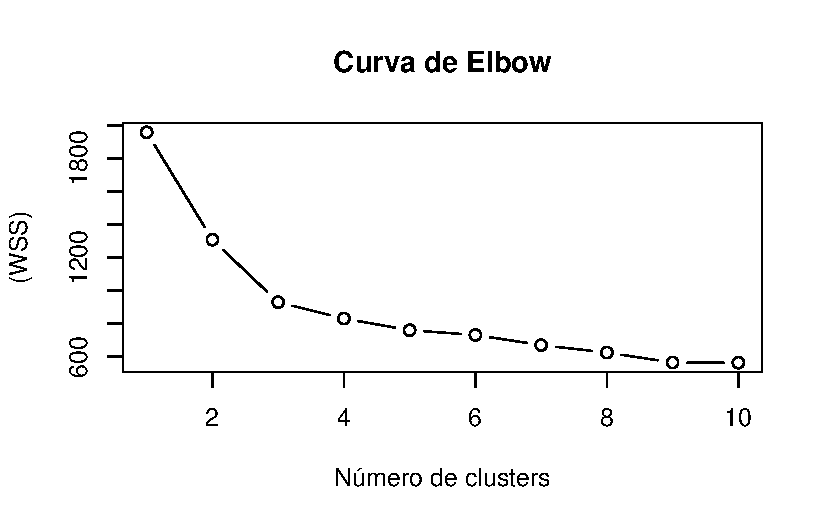
\includegraphics{wines_analysis_files/figure-pdf/unnamed-chunk-26-1.pdf}

Ao analisar a curva de elbow relativa aos componentes principais, nos
parece claro que há uma tendência à escolha de \(k=3\), vez que
observa-se a formação do ``cotovelo'' neste ponto.

Isto demonstra o bom ajuste dos componentes principais aos dados
originais, haja vista que o conjunto de dados inicial wine possui uma
variável categórica, qual seja Cultivars, que dividia o conjunto em 3
classes distintas.

É salutar ressaltar que esta variável não foi considerada tanto na
análise de componentes principais da Secção anterior, quanto nesta
clusterização, para que não viesse a interferir nas análises.

Ante o exposto, \textbf{caso optassemos por seguir o método da curva de
elbow para definição de \(k\) no \(k\)-Means, escolheríamos \(k=3\).}

Vejamos a seguir o que o silhouette score tem a nos dizer:

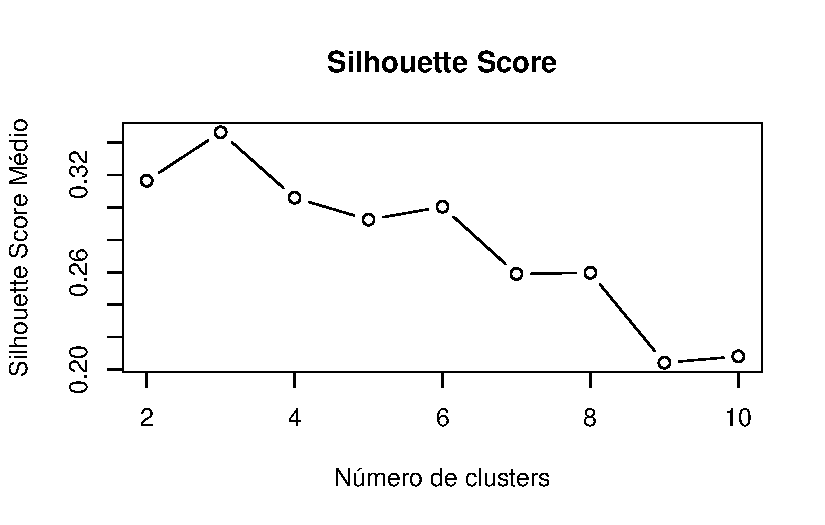
\includegraphics{wines_analysis_files/figure-pdf/unnamed-chunk-27-1.pdf}

Neste ponto a lógica inverte-se: Se para a curva de elbow melhor seria o
valor de \(k\) quanto menor fosse o valor no eixo \(y\) do gráfico, para
o silhouette score quanto mais elevado for o valor apontado pelo eixo
\(y\) do gráfico, mais ajustado aos dados será o número de \(k\)
proposto.

\textbf{É possível portanto enxergar que o silhouette score confirma a
tendência apontada anteriormente na curva de elbow, e demonstra que
devemos inicializar o \(k\)-Means em \(K=3\) para obter um resultado que
seja o mais próximo possível do ideal quando do agrupamento dos dados.}

\newpage{}

\paragraph{Realização do K-Means com
K=3:}\label{realizauxe7uxe3o-do-k-means-com-k3}

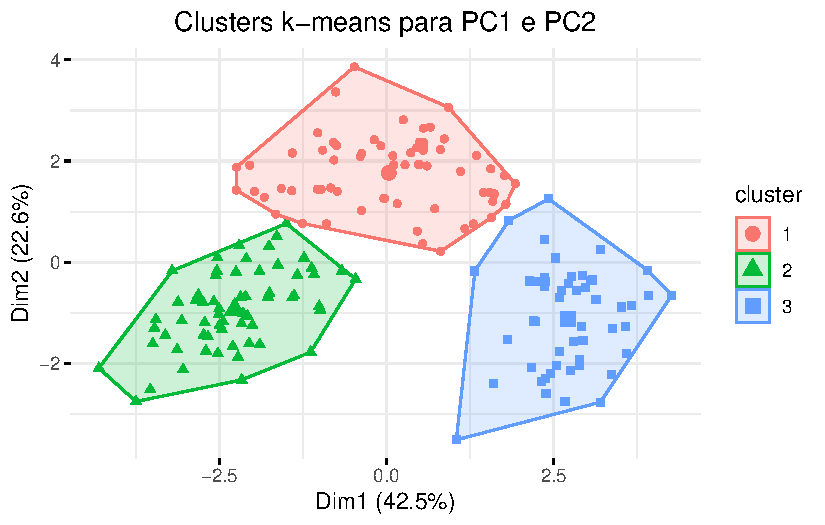
\includegraphics{wines_analysis_files/figure-pdf/unnamed-chunk-29-1.pdf}

\textbf{Informações importantes a respeito da visualização anterior:}

\begin{quote}
DIM1 (Eixo X) e DIM2 (Eixo Y): Estes são os dois primeiros componentes
principais derivados do PCA. DIM1 diz respeito ao componente principal
que captura a maior parte da variação dos dados, seguido por DIM2.
\end{quote}

\begin{quote}
Percentagens associadas às dimensões: Estas porcentagens indicam a
quantidade de variação dos dados originais explicada por cada componente
principal. No caso em tela, DIM1 explica 42,5\% da variância total nos
dados e DIM2 explica 22,6\%. Juntos, esses dois componentes principais
explicam 65,1\% da variância total dos dados.
\end{quote}

\begin{quote}
\textbf{Distribuição dos pontos dentro dos clusters:} Observa-se pela
maneira em que os pontos estão distribuídos dentro das elipses que há um
ótimo nível de compactação e coesão dos clusters. Vale mencionar a
excelente definição do cluster 2, onde a maior parte dos pontos aparecem
próximos ao centroide.
\end{quote}

\begin{quote}
\textbf{Separação dos clusters:} Depreende-se da análise do gráfico que
os clusters estão bem definidos e claramente separados, o que constitui
um indicativo de que o k-means se saiu bem na tarefa de identificação de
grupos distintos nos dados.
\end{quote}

\newpage{}

\subparagraph{Análise das medidas de
avaliação}\label{anuxe1lise-das-medidas-de-avaliauxe7uxe3o}

Apresentaremos a seguir as medidas de avaliação que serão utilizadas
para comparar as diferentes aplicações do K-Means, tanto aos dados
originais quanto aos componentes principais oriundos dos dados, conforme
a presente Secção.

Não teceremos comentários sobre estes números neste momento, pois eles
servirão de base comparativa com as demais soluções. Na Secção da
conclusão retornaremos a eles.

\begingroup\fontsize{12}{14}\selectfont

\begin{longtable}[t]{lrrr}
\caption{\label{tab:unnamed-chunk-30}Resumo dos WithinSS do K-means em K=3}\\
\toprule
  & Cluster1 & Cluster2 & Cluster3\\
\midrule
\cellcolor{gray!15}{Cluster} & \cellcolor{gray!15}{1.0000} & \cellcolor{gray!15}{2.0000} & \cellcolor{gray!15}{3.0000}\\
WithinSS & 408.8896 & 280.7431 & 239.7935\\
\bottomrule
\end{longtable}
\endgroup{}

\begingroup\fontsize{12}{14}\selectfont

\begin{longtable}[t]{rrrr}
\caption{\label{tab:unnamed-chunk-30}Resumo Agregado do K-means em K=3}\\
\toprule
TotalSS & TotalWithinSS & BetweenSS & VarianciaExplicada\\
\midrule
\cellcolor{gray!15}{1958.108} & \cellcolor{gray!15}{929.4262} & \cellcolor{gray!15}{1028.681} & \cellcolor{gray!15}{52.53447}\\
\bottomrule
\end{longtable}
\endgroup{}

Ante todo o exposto é possível dizer que o algoritmo K-means aplicado
aos 6 componentes principais derivados dos dados originais apresentou
boa performance na tarefa de agrupamento desses dados, o que demonstra o
poder de se aliar as duas técnicas para reduzir a dimensionalidade dos
dados quando estes apresentam elevado número de atributos e,
posteriormente, segmentá-los de maneira coesa e eficiente.

\paragraph{4.2.1.2 - Aplicação do K-Means aos dados originais
standardizados:}\label{aplicauxe7uxe3o-do-k-means-aos-dados-originais-standardizados}

\begingroup\fontsize{3.5}{5.5}\selectfont

\begin{longtable}[t]{r>{\raggedleft\arraybackslash}p{1cm}rrrrrrrrrrr}
\caption{\label{tab:unnamed-chunk-31}Dados standardizados}\\
\toprule
Alcohol & Malic\_Acid & Ash & Ash\_Alcanity & Magnesium & Total\_Phenols & Flavanoids & Nonflavanoid\_Phenols & Proanthocyanins & Color\_Intensity & Hue & OD280 & Proline\\
\midrule
\cellcolor{gray!15}{1.5143408} & \cellcolor{gray!15}{-0.5606682} & \cellcolor{gray!15}{0.2313998} & \cellcolor{gray!15}{-1.1663032} & \cellcolor{gray!15}{1.9085215} & \cellcolor{gray!15}{0.8067217} & \cellcolor{gray!15}{1.0319081} & \cellcolor{gray!15}{-0.6577078} & \cellcolor{gray!15}{1.2214385} & \cellcolor{gray!15}{0.2510088} & \cellcolor{gray!15}{0.3611585} & \cellcolor{gray!15}{1.8427215} & \cellcolor{gray!15}{1.0101594}\\
0.2455968 & -0.4980086 & -0.8256672 & -2.4838405 & 0.0180940 & 0.5670481 & 0.7315653 & -0.8184106 & -0.5431887 & -0.2924962 & 0.4049085 & 1.1103172 & 0.9625263\\
\cellcolor{gray!15}{0.1963252} & \cellcolor{gray!15}{0.0211715} & \cellcolor{gray!15}{1.1062139} & \cellcolor{gray!15}{-0.2679823} & \cellcolor{gray!15}{0.0881098} & \cellcolor{gray!15}{0.8067217} & \cellcolor{gray!15}{1.2121137} & \cellcolor{gray!15}{-0.4970050} & \cellcolor{gray!15}{2.1299594} & \cellcolor{gray!15}{0.2682629} & \cellcolor{gray!15}{0.3174085} & \cellcolor{gray!15}{0.7863692} & \cellcolor{gray!15}{1.3912237}\\
1.6867914 & -0.3458351 & 0.4865539 & -0.8069748 & 0.9282998 & 2.4844372 & 1.4623994 & -0.9791134 & 1.0292513 & 1.1827317 & -0.4263410 & 1.1807407 & 2.3280068\\
\cellcolor{gray!15}{0.2948684} & \cellcolor{gray!15}{0.2270533} & \cellcolor{gray!15}{1.8352256} & \cellcolor{gray!15}{0.4506745} & \cellcolor{gray!15}{1.2783790} & \cellcolor{gray!15}{0.8067217} & \cellcolor{gray!15}{0.6614853} & \cellcolor{gray!15}{0.2261576} & \cellcolor{gray!15}{0.4002753} & \cellcolor{gray!15}{-0.3183774} & \cellcolor{gray!15}{0.3611585} & \cellcolor{gray!15}{0.4483365} & \cellcolor{gray!15}{-0.0377675}\\
\addlinespace
1.4773871 & -0.5159113 & 0.3043010 & -1.2860793 & 0.8582840 & 1.5576991 & 1.3622851 & -0.1755994 & 0.6623487 & 0.7298108 & 0.4049085 & 0.3356589 & 2.2327407\\
\bottomrule
\end{longtable}
\endgroup{}

Na Secção 4.2.1.1 realizamos o agrupamento dos 6 componentes principais
retidos dos dados originais. Para tanto, utilizamos apenas o algoritmo
K-Means na tarefa de clusterização.

De agora em diante retornaremos aos dados originais, com o fito de
observar se os resultados obtidos no agrupamento serão melhores ou ao
menos tão satisfatórios quanto aqueles obtidos após a aplicação da ACP.

Ademais, faremos uso do data set original sem a variável categórica
Cultivars, que encontra-se armazenado na variável
``wine\_clean\_subset'' no relatório em R. Entretanto, realizaremos a
standardização desses dados, uma vez que tal procedimento demonstrou-se
fundamental quando da análise exposta na Secção 4.1 do presente
relatório, pois os dados possuem variáveis com escalas muito diferentes,
o que demonstrou ter um impactos significativos na performance de
algoritmos que não lidam bem com esse tipo de informação, como é o caso
dos algoritmos utilizados na análise de clusters.

Além do K-Means, para estes testes utilizaremos também a análise de
clusters hierárquica de modo a perceber qual apresentará melhor
resultado ou se os resultados de uma confirmam aquilo que fora
encontrado na outra.

\subparagraph{\texorpdfstring{\textbf{Definição do número ideal de
clusters por meio da aplicação das técnicas do silhouette score e curva
de
elbow.}}{Definição do número ideal de clusters por meio da aplicação das técnicas do silhouette score e curva de elbow.}}\label{definiuxe7uxe3o-do-nuxfamero-ideal-de-clusters-por-meio-da-aplicauxe7uxe3o-das-tuxe9cnicas-do-silhouette-score-e-curva-de-elbow.-1}

A seguir observaremos o comportamento da curva de elbow e do silhouette
score para nos ajudar a definir \(k\) na inicialização do K-Means.

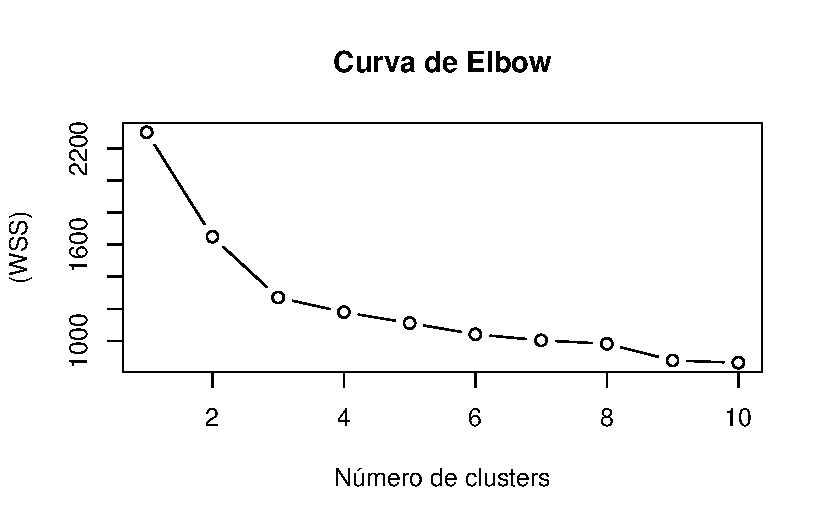
\includegraphics{wines_analysis_files/figure-pdf/unnamed-chunk-32-1.pdf}

Ao analisar a curva de elbow relativa aos componentes principais, mais
uma vez há uma clara tendência à escolha de \(k=3\), vez que observa-se
a formação do ``cotovelo'' neste ponto. Entretanto, seguindo este método
não nos parece errado também a solução com \(k=4\).

Ante o exposto, \textbf{caso optassemos por seguir o método da curva de
elbow para definição de \(k\) no \(k\)-Means, escolheríamos \(k=3\) ou
\(k=4\).}

Utilizaremos portanto o silhouette score para saber se há necessidade de
testar a solução com \(k=4\) ou se a diferença para \(k=3\) será muito
nítida neste método.

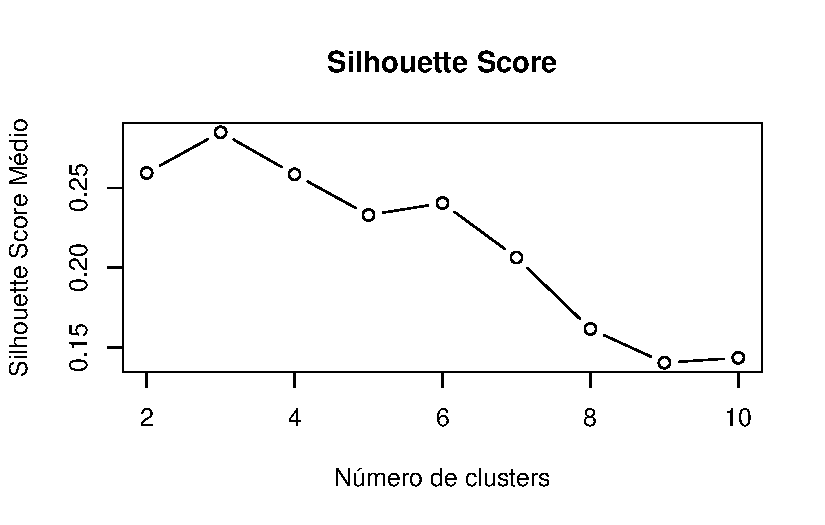
\includegraphics{wines_analysis_files/figure-pdf/unnamed-chunk-33-1.pdf}

Podemos enxergar que o silhouette score demonstra que \(k=3\) tende a
ser a solução mais próxima do ideal na aplicação do k-means aos dados
originais standardizados.

A queda abrupta nos valores do silhouette score médio quando passamos de
3 para 4 nos diz que muito provavelmente não será uma boa solução optar
por \(k=4\).

\textbf{Desta feita, antes de apontar \(k=3\) como a melhor solução,
analisaremos os números relativos à coesão intra-cluster e à
heterogeneidade entre os grupos para decidir sobre a melhor solução.}

\paragraph{Medidas de Avaliação do
K-means}\label{medidas-de-avaliauxe7uxe3o-do-k-means}

Apresentamos a seguir uma rápida explanação sobre as medidas que serão
utilizadas para comparar a performance de cada k-means desenvolvido.

\begin{itemize}
\item
  \textbf{TotSS (Total Sum of Squares)} A soma total dos quadrados
  (TotSS) representa a variabilidade total presente nos dados originais.
  É a soma das distâncias quadráticas de cada ponto até a média global
  dos dados. Essa medida fornece uma visão geral da dispersão total dos
  dados antes de qualquer análise de clusters.
\item
  \textbf{TotalWithinSS (Total Within-Cluster Sum of Squares)} A soma
  total dos quadrados dentro dos clusters (TotalWithinSS) é a soma das
  distâncias quadráticas de cada ponto até o centro do seu respectivo
  cluster, somada para todos os clusters. Aqui, quanto menor o valor,
  mais compactos e homogêneos e melhores são os clusters.
\item
  \textbf{WithinSS (Within-Cluster Sum of Squares)} A soma dos quadrados
  dentro do cluster (WithinSS) é calculada individualmente para cada
  cluster. Representa a variabilidade dentro de um cluster específico,
  medindo o quão dispersos estão os pontos em relação ao centro do
  cluster. Valores menores indicam clusters mais compactos e portanto
  melhores.
\item
  \textbf{BetweenSS (Between-Cluster Sum of Squares)} A soma dos
  quadrados entre os clusters (BetweenSS) é a soma das distâncias
  quadráticas entre os centros dos clusters e a média global dos dados,
  ponderada pelo número de pontos em cada cluster. Esta medida reflete a
  separação entre os clusters; valores maiores indicam clusters mais bem
  separados e heterogêneos entre si.
\item
  \textbf{Percentagem de Variância Explicada} A variância explicada é a
  percentagem da variabilidade total (TotSS) que é explicada pela
  divisão dos dados em clusters. É calculada como a razão entre
  BetweenSS e TotSS, multiplicada por 100. Essa medida indica o quão bem
  os clusters formados explicam a variabilidade dos dados originais.
  Valores maiores sugerem uma melhor divisão dos dados em clusters,
  capturando mais da estrutura inerente aos dados.
\end{itemize}

\paragraph{Aplicação do K-Means com K=3 para os dados originais
standardizados:}\label{aplicauxe7uxe3o-do-k-means-com-k3-para-os-dados-originais-standardizados}

Além da definição do número de clusters a serem utilizados no algoritmo,
o K-Means também necessita de outro parâmetro para sua correta
aplicação: o n\_start.

O hiperparâmetro \texttt{nstart} no algoritmo k-means é responsável por
controlar o número de inicializações aleatórias que o algoritmo tentará
para encontrar os centróides iniciais. Em outras palavras, ele define
quantas vezes o algoritmo irá iniciar o processo de agrupamento a partir
de diferentes conjuntos aleatórios de centróides.

Neste ponto, quanto maior o valor de \texttt{nstart}, maior a
probabilidade de o algoritmo encontrar uma solução globalmente melhor,
mas isso também poderá afetar consideravelmente o tempo de execução.
Portanto, a exemplo do que fizemos na Secção 4.2.1.1, onde utilizamos
n\_start=25, aplicaremos o mesmo aqui.

\textbf{A seguir, os números associados a \(k=3\):}

\begingroup\fontsize{12}{14}\selectfont

\begin{longtable}[t]{lrrr}
\caption{\label{tab:unnamed-chunk-35}Resumo dos Clusters do K-means em K=3}\\
\toprule
  & Cluster1 & Cluster2 & Cluster3\\
\midrule
\cellcolor{gray!15}{Cluster} & \cellcolor{gray!15}{1.0000} & \cellcolor{gray!15}{2.0000} & \cellcolor{gray!15}{3.0000}\\
WithinSS & 558.6971 & 385.6983 & 326.3537\\
\bottomrule
\end{longtable}
\endgroup{}

\begingroup\fontsize{12}{14}\selectfont

\begin{longtable}[t]{rrrr}
\caption{\label{tab:unnamed-chunk-35}Resumo Agregado do K-means em K=3}\\
\toprule
TotSS & TotalWithinSS & BetweenSS & Variancia\_Explicada\\
\midrule
\cellcolor{gray!15}{2301} & \cellcolor{gray!15}{1270.749} & \cellcolor{gray!15}{1030.251} & \cellcolor{gray!15}{44.77405}\\
\bottomrule
\end{longtable}
\endgroup{}

\textbf{De outro giro, quando definimos \(k=4\), estes são os
indicadores para avaliação:}

\begingroup\fontsize{12}{14}\selectfont

\begin{longtable}[t]{lrrrr}
\caption{\label{tab:unnamed-chunk-37}Resumo dos Clusters do K-means em K=4}\\
\toprule
  & Cluster1 & Cluster2 & Cluster3 & Cluster4\\
\midrule
\cellcolor{gray!15}{Cluster} & \cellcolor{gray!15}{1.0000} & \cellcolor{gray!15}{2.0000} & \cellcolor{gray!15}{3.0000} & \cellcolor{gray!15}{4.0000}\\
WithinSS & 307.0966 & 268.5747 & 302.9915 & 289.9515\\
\bottomrule
\end{longtable}
\endgroup{}

\begingroup\fontsize{12}{14}\selectfont

\begin{longtable}[t]{rrrr}
\caption{\label{tab:unnamed-chunk-37}Resumo Agregado do K-means em K=4}\\
\toprule
TotSS & TotalWithinSS & BetweenSS & Variancia\_Explicada\\
\midrule
\cellcolor{gray!15}{2301} & \cellcolor{gray!15}{1168.614} & \cellcolor{gray!15}{1132.386} & \cellcolor{gray!15}{49.21276}\\
\bottomrule
\end{longtable}
\endgroup{}

\paragraph{\texorpdfstring{Comparação das Medidas de Avaliação para
\(K=3\) e
\(K=4\)}{Comparação das Medidas de Avaliação para K=3 e K=4}}\label{comparauxe7uxe3o-das-medidas-de-avaliauxe7uxe3o-para-k3-e-k4}

\begin{itemize}
\tightlist
\item
  \textbf{TotSS (Total Sum of Squares)}

  \begin{itemize}
  \tightlist
  \item
    \(K=3\): 23011
  \item
    \(K=4\): 23011
  \item
    \textbf{Interpretação:} A TotSS é a mesma para \(K=3\) e \(K=4\),
    pois representa a variabilidade total dos dados originais e
    independe do número de clusters.
  \end{itemize}
\item
  \textbf{TotalWithinSS (Total Within-Cluster Sum of Squares)}

  \begin{itemize}
  \tightlist
  \item
    \(K=3\): 1270.749
  \item
    \(K=4\): 1168.614
  \item
    \textbf{Interpretação:} O TotalWithinSS é menor para \(K=4\), o que
    indica que os clusters são mais homogéneos em \(K=4\).
  \end{itemize}
\item
  \textbf{WithinSS (Within-Cluster Sum of Squares)}

  \begin{itemize}
  \tightlist
  \item
    \(K=3\): {[}558.697, 385.698, 326.354{]}
  \item
    \(K=4\): {[}307.097, 268.575, 302.992, 289.952{]}
  \item
    \textbf{Interpretação:} Cada cluster individualmnege considerado em
    \(K=4\) possui um WithinSS menor ou comparável aos clusters em
    \(K=3\), indicando novamente melhores números para \(K=4\).
  \end{itemize}
\item
  \textbf{BetweenSS (Between-Cluster Sum of Squares)}

  \begin{itemize}
  \tightlist
  \item
    \(K=3\): 1030.251
  \item
    \(K=4\): 1132.386
  \item
    \textbf{Interpretação:} O BetweenSS é maior para \(K=4\), o que
    sugere que os clusters estão mais bem separados quando optamos por 4
    clusters.
  \end{itemize}
\item
  \textbf{Variância Explicada}

  \begin{itemize}
  \tightlist
  \item
    \(K=3\): 44.774\%
  \item
    \(K=4\): 49.213\%
  \item
    \textbf{Interpretação:} A variância explicada é maior em \(K=4\), de
    modo a apontar que a divisão dos dados em 4 clusters captura de
    maneira mais fidedigna a estrutura dos dados originais.
  \end{itemize}
\end{itemize}

Por fim, com base nas medidas supramencionadas, \(K=4\) parece ser a
melhor escolha. Isso porque o TotalWithinSS é menor, o BetweenSS é
maior, e a variância explicada é mais alta, indicando que provavelmente
os clusters em \(K=4\) são mais coesos internamente, melhor separados, e
capturam mais da variabilidade dos dados.

Isto contradiz os números apresentados pela curva de elbow e silhouette
score, que apontavam para \(k=3\) como a melhor solução.

\textbf{Passaremos a seguir à clusterização hierárquica de modo a
dirimir eventuais dúvidas e concluir aquele que parece ser o melhor
desfecho para agrupar e segmentar os dados do data set wine, vez que a
principal vantagem deste método sobre o K-Means diz respeito a não haver
necessidade de se definir arbitrariamente o número de \(K\) antes de
inicializar o algoritmo.}

\paragraph{4.2.1.3 - Aplicação da clusterização hieráquica aos dados
originais
standardizados:}\label{aplicauxe7uxe3o-da-clusterizauxe7uxe3o-hieruxe1quica-aos-dados-originais-standardizados}

A clusterização hierárquica é um método de agrupamento de dados que cria
uma hierarquia de clusters, onde cada ponto começa como um cluster
individual e é agrupado em clusters maiores à medida que o algoritmo
prossegue. As vantagens desse método recaem sobre a sua capacidade de
criar uma visão global da estrutura dos dados, sem a necessidade de
especificar previamente o número de clusters, além da capacidade de
representar clusters aninhados, o que pode ser útil em conjuntos de
dados com estruturas complexas ou desconhecidas.

\newpage{}

\subparagraph{Métodos de aplicação da análise de Clusters
hierárquica:}\label{muxe9todos-de-aplicauxe7uxe3o-da-anuxe1lise-de-clusters-hieruxe1rquica}

\begin{itemize}
\tightlist
\item
  \textbf{Single Linkage (ligação única):}

  \begin{itemize}
  \tightlist
  \item
    Baseia-se na distância mínima entre os pontos de dois clusters.
  \item
    A distância entre dois clusters é definida como a menor distância
    entre qualquer par de pontos, um de cada cluster.
  \item
    Tende a formar clusters alongados, sensíveis a ruídos e outliers.
  \end{itemize}
\item
  \textbf{Average Linkage (ligação média):}

  \begin{itemize}
  \tightlist
  \item
    Calcula a média das distâncias entre todos os pares de pontos, um de
    cada cluster.
  \item
    Menos sensível a outliers do que a ligação única.
  \item
    Pode resultar em clusters mais compactos e equilibrados.
  \end{itemize}
\item
  \textbf{Complete Linkage (ligação completa):}

  \begin{itemize}
  \tightlist
  \item
    Baseia-se na distância máxima entre os pontos de dois clusters.
  \item
    A distância entre dois clusters é definida como a maior distância
    entre qualquer par de pontos, um de cada cluster.
  \item
    Tende a produzir clusters mais compactos e esféricos, menos
    sensíveis a outliers do que a ligação única.
  \end{itemize}
\end{itemize}

Para facilitar o entendimento destes métodos, observemos a imagem a
seguir:

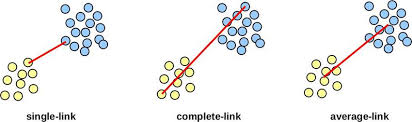
\includegraphics{/Users/pedroh.mello/Desktop/MESTRADO_MCDE/ML NAO SUPERVISIONADO/PROJETO_FINAL/img_linkages.jpeg}!

\newpage{}

\subparagraph{Análise dos dendogramas para cada
método:}\label{anuxe1lise-dos-dendogramas-para-cada-muxe9todo}

\subparagraph{Dendograma - Single
Linkage}\label{dendograma---single-linkage}

\begin{figure}[H]

{\centering 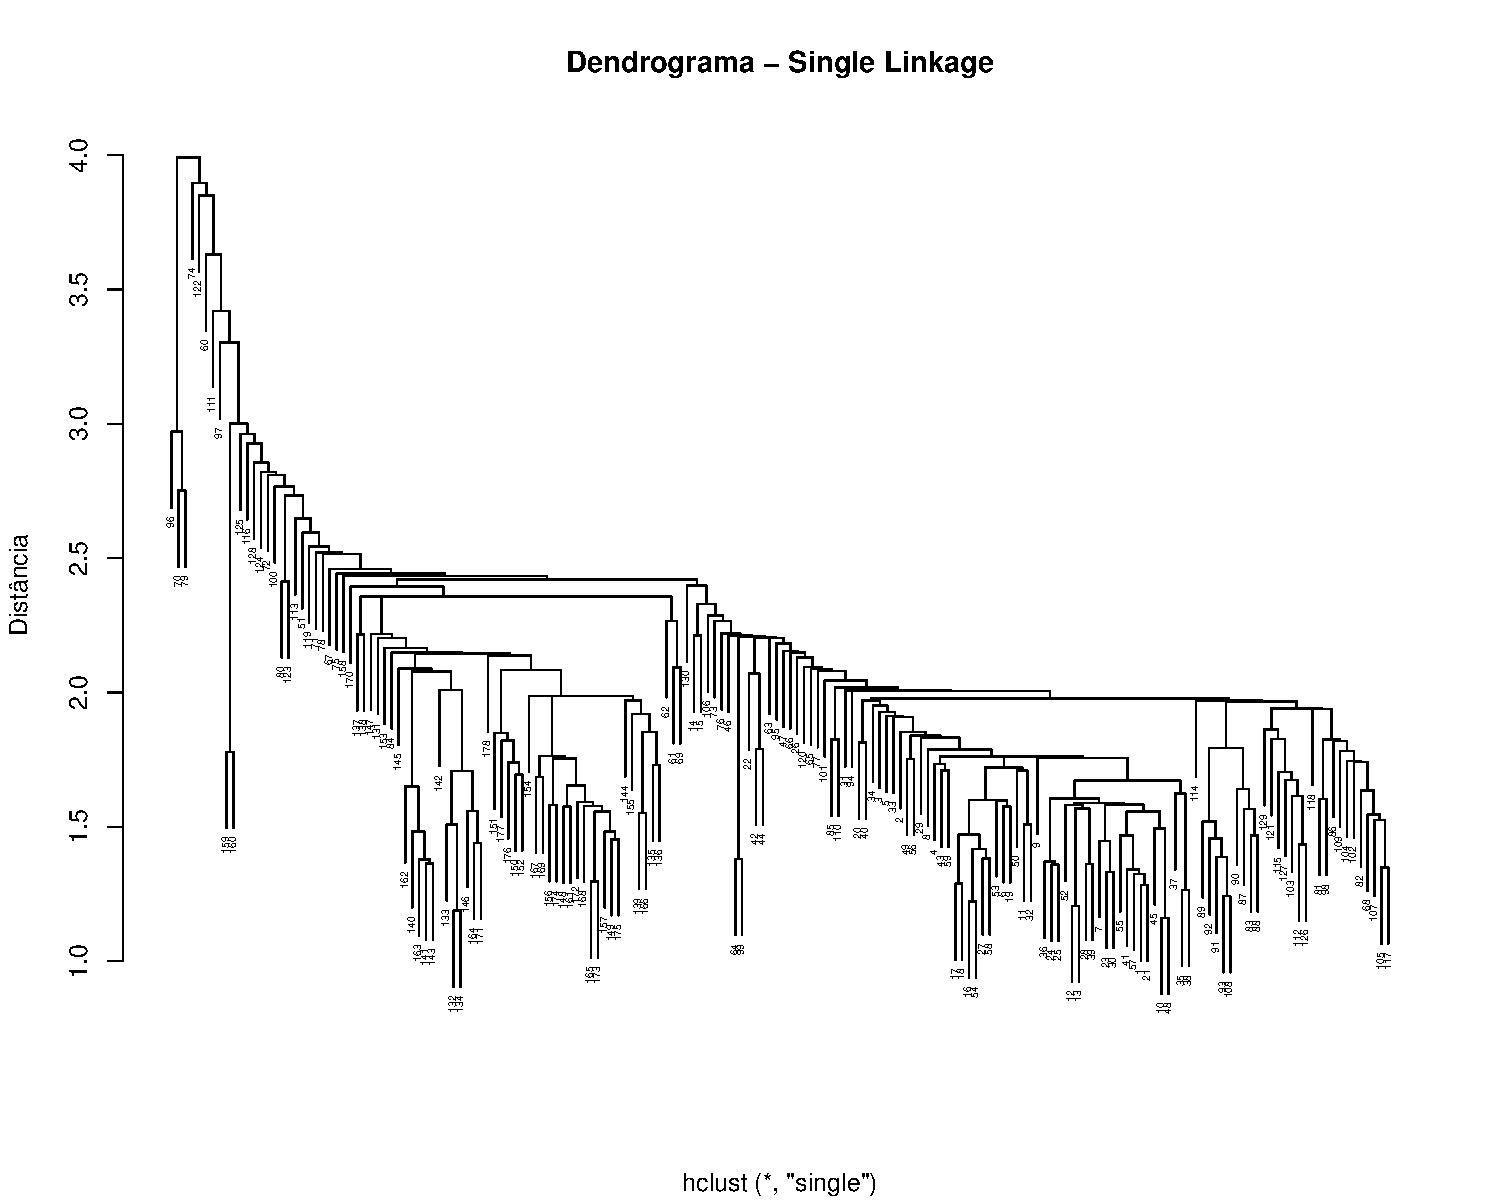
\includegraphics{wines_analysis_files/figure-pdf/unnamed-chunk-38-1.pdf}

}

\caption{Clusters em single linkage}

\end{figure}%

O método single linkage aplicado aos dados wine standardizados não
apresentou bons resultados. Conforme é possível notar, se comparado aos
demais métodos esse foi o que produziu os clusters mais desequilibrados
e sensíveis a outliers, não constituindo um bom indicador.

\newpage{}

\subparagraph{Dendograma - Average
Linkage}\label{dendograma---average-linkage}

\begin{figure}[H]

{\centering 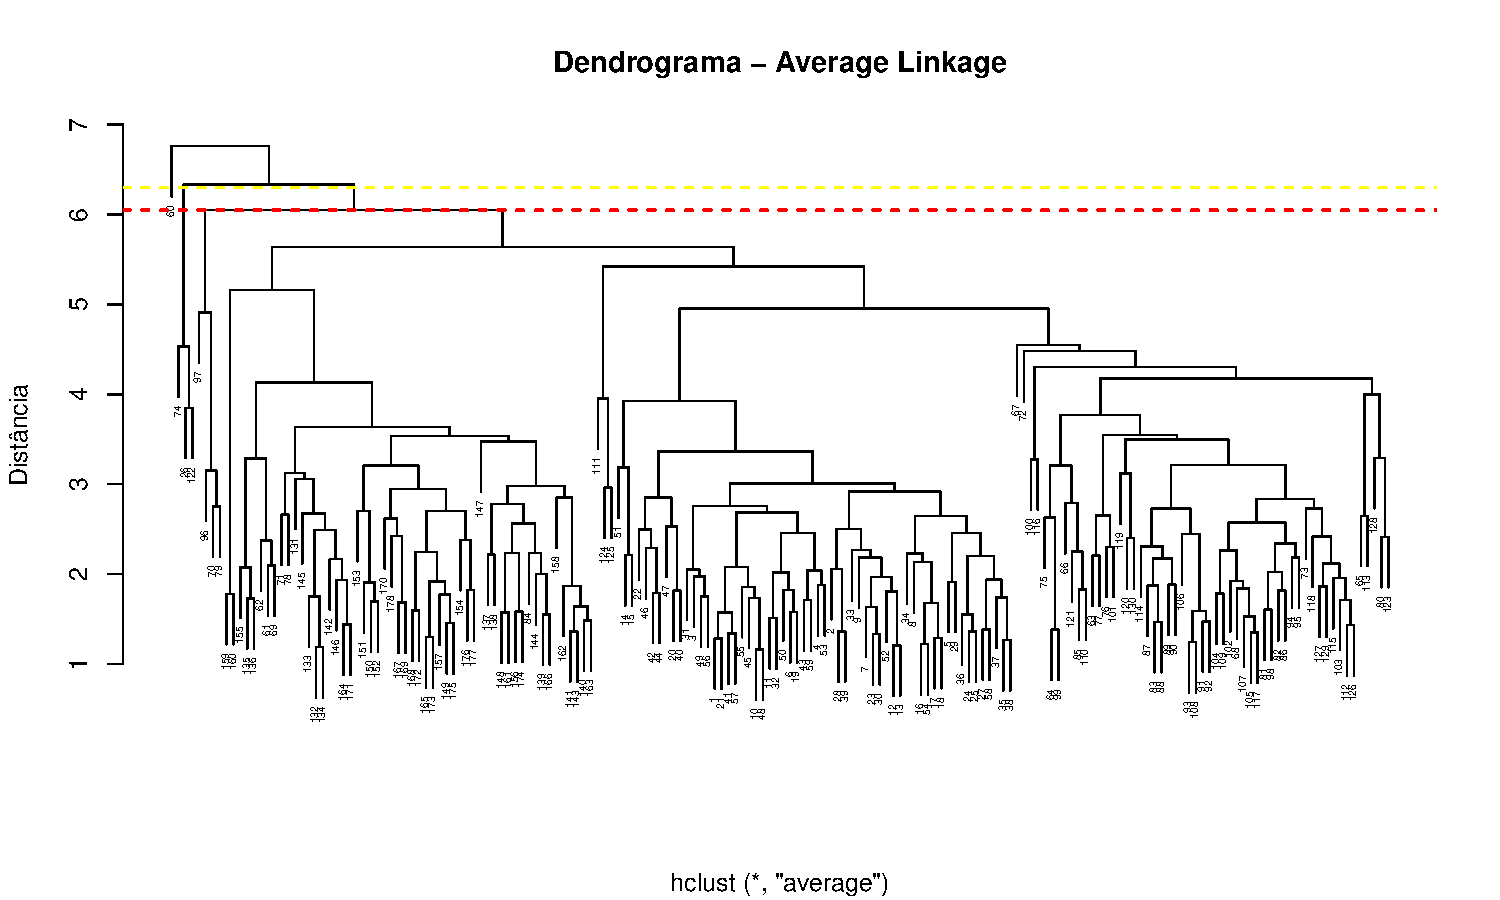
\includegraphics{wines_analysis_files/figure-pdf/unnamed-chunk-39-1.pdf}

}

\caption{Em Amarelo: 3 clusters; Em Vermelho: 4 clusters}

\end{figure}%

Apresentou rrsultados melhores se comparados ao single linkage,
entretanto ainda não parece bom o suficiente pois produziu grupos ainda
desequilibrados.

Além disso, como podemos ver ele quase não demonstra diferença na altura
ao escolhermos 3 ou 4 clusters, o que não seria bom para a análise.

\newpage{}

\subparagraph{Dendograma - Complete
Linkage}\label{dendograma---complete-linkage}

\begin{figure}[H]

{\centering 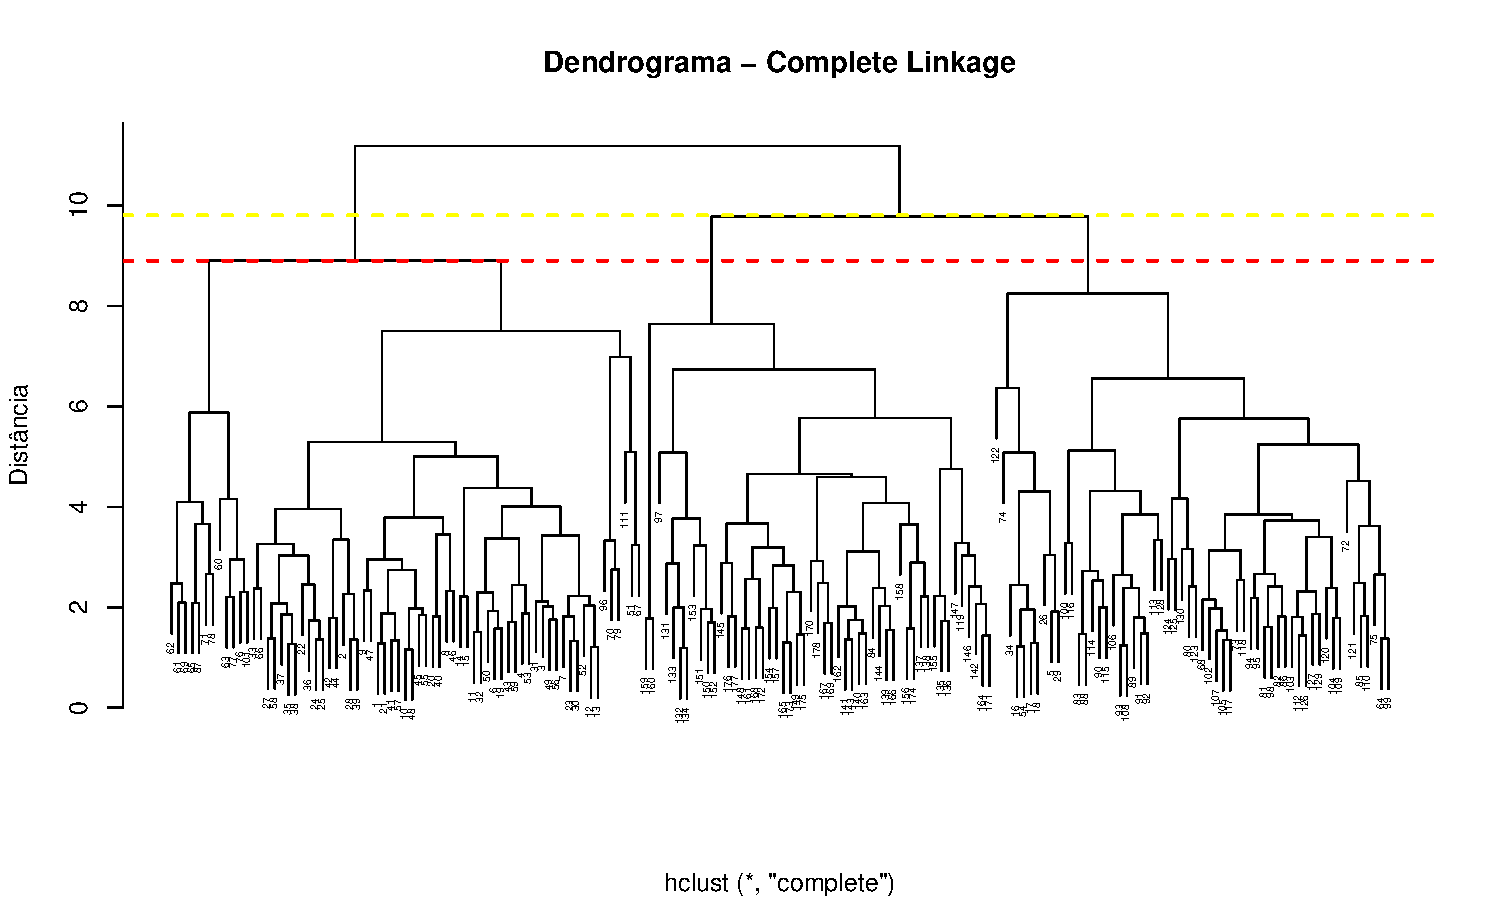
\includegraphics{wines_analysis_files/figure-pdf/unnamed-chunk-40-1.pdf}

}

\caption{Em Amarelo: 3 clusters; Em Vermelho: 4 clusters}

\end{figure}%

Apesar de ainda não ser o idela, o complete linkage com o corte no nível
de 4 grupos parece ser aquele que produz os grupos com maior coesão
interna e distância dos demais.

Isto confirma aquilo que fora aventado anteriormente no K-Means, de modo
a demonstrar que a melhor solução para os dados aqui propostos, qual
seja o conjunto de dados original standardizado, seria a partição em 4
clusters.

Entretanto, conforme veremos a seguir, a clusterização hierárquica via
complete linkage ainda não nos pareceu melhor que o K-Means aplicado aos
componentes principais realizada na Secção 4.2.1.1 deste trabalho, vez
que a definição dos grupos parece mais desequilibrada aqui nos clusters
hierárquicos, a saber:

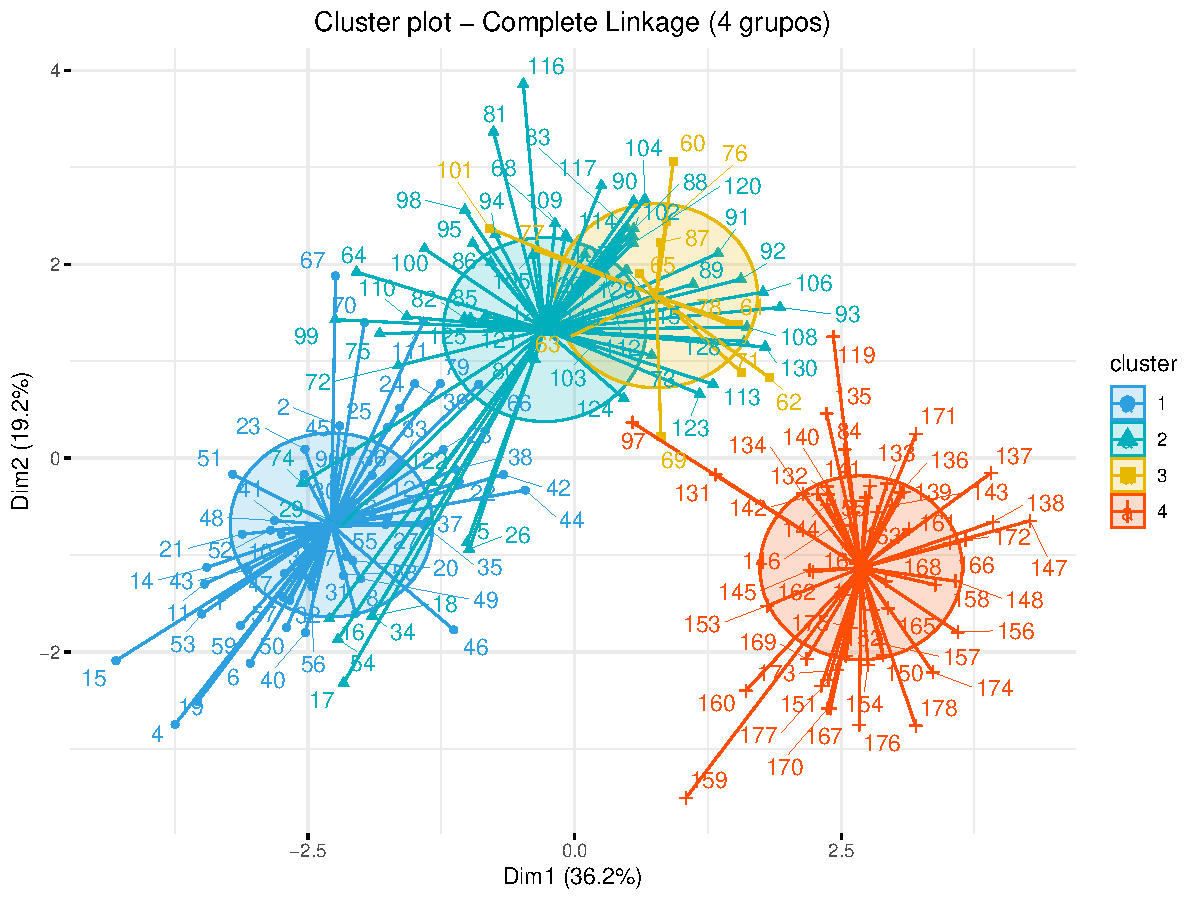
\includegraphics{wines_analysis_files/figure-pdf/unnamed-chunk-41-1.pdf}

\subsection{Conclusões}\label{conclusuxf5es}

A análise realizada demonstrou que a combinação dos métodos de Análise
de Componentes Principais (PCA) e k-means resultou na melhor solução
para a segmentação dos dados. Especificamente, o k-means com \(k = 3\)
sobre os componentes principais provou ser a abordagem mais eficaz. Esta
combinação de métodos permitiu uma análise mais precisa e uma melhor
separação dos clusters, comparando com outras abordagens testadas. A
utilização de 6 componentes principais foi justificada pela captura de
85\% da variância total dos dados, o que facilitou a interpretação e
reduziu a dimensionalidade sem perda significativa de informação.

A escolha de \(k = 3\) em vez de \(k = 4\) foi justificada através de
uma análise detalhada das métricas de avaliação dos clusters. Apesar de
\(k = 4\) ter mostrado uma menor soma total dos quadrados dentro dos
clusters (TotalWithinSS) e uma maior soma dos quadrados entre os
clusters (BetweenSS), indicando clusters mais homogéneos internamente e
mais separados entre si, a decisão final foi influenciada pela análise
da curva de elbow e do silhouette score. A curva de elbow, que ajuda a
identificar o ponto onde adicionar mais clusters deixa de proporcionar
ganhos significativos na explicação da variância, sugeriu que \(k = 3\)
era o ponto ideal, além do silhouette score, que mede quão semelhantes
os objetos são ao seu próprio cluster em comparação ao cluster mais
próximo, também ter indicado melhor desempenho para \(k = 3\). Estas
análises indicam que, embora \(k = 4\) pudesse oferecer uma ligeira
melhora nas métricas internas dos clusters, \(k = 3\) proporciona um
balanço mais adequado entre coesão interna e separação entre clusters,
garantindo uma segmentação eficiente e significativa dos dados.

Esta conclusão é apoiada pelas métricas de avaliação utilizadas, que
mostraram que os números obtidos com a combinação de PCA e k-means foram
superiores aos de outras combinações de métodos. Portanto, a aplicação
dessas técnicas não supervisionadas demonstrou ser eficaz na análise e
segmentação dos dados do conjunto de vinhos, contribuindo para uma
melhor compreensão das características que distinguem os diferentes
tipos de vinhos analisados.

\textbf{O código fonte em R do presente trabalho consta ao link do
reposiório a seguir:
\href{https://github.com/mello-pedro/SUPERV_ML_MCDE_23_24/blob/main/R_SOURCE_CODE_BIKE_SHARING.qmd}{Repositório
GitHub}.}



\end{document}
